%----------------------------------------------------------------
%
%  File    :  thesis.tex
%
%  Authors :  David Lechner, FH Campus Wien, Austria
%
%  Created :  10 Oct 2019
%
%  Changed :  10 Oct 2019
%
%----------------------------------------------------------------


% --- General Setup ---------------------------------------------
% !TEX encoding = IsoLatin2
\documentclass[11pt,a4paper,oneside]{scrbook}
\usepackage[T1]{fontenc}
\usepackage[utf8]{inputenc}

\usepackage[ngerman]{babel}

% for nicer PDF rendering. Alternatively, when using MikTeX,
% you could also manually install the cm-super package
\usepackage{lmodern}

\usepackage[T1]{fontenc}

% want Arial? uncomment next two lines...
%\usepackage{uarial}
%\renewcommand{\familydefault}{\sfdefault}

\usepackage{caption}
\usepackage{subcaption}

\usepackage{url}

\usepackage{latexsym}

\usepackage{geometry} % define pagesize in more detail

\usepackage{fancyhdr} % nicer headers and footers

\usepackage{colortbl} % define colored backgrounds for tables

\usepackage{makecell}

\usepackage{multirow}

\usepackage{siunitx}

\usepackage{eurosym}

\usepackage{longtable}


\DeclareFontEncoding{LS1}{}{}
\DeclareFontSubstitution{LS1}{stix}{m}{n}
\DeclareRobustCommand{\diameter}{
    \text{\usefont{LS1}{stixscr}{m}{n}\symbol{"60}}
}

\usepackage{amsmath}

% \usepackage{tikzpagenodes}

\usepackage{courier} %for listings
\usepackage{listings} % nicer code formatting
\lstset{basicstyle=\ttfamily,breaklines=true}

  \usepackage[pdftex]{graphicx}
  \DeclareGraphicsExtensions{.pdf,.jpg,.png}
  \pdfcompresslevel=9
  \pdfpageheight=297mm
  \pdfpagewidth=210mm
  \usepackage[         % hyperref should be last package loaded
    pdftex,
    bookmarks,
    bookmarksnumbered,
    linktocpage,
    pagebackref,
    pdfview={Fit},
    pdfstartview={Fit},
    hidelinks,
    pdfpagemode=UseOutlines,                 % open bookmarks in Acrobat
  ]{hyperref}
  \usepackage{bookmark}

\geometry{a4paper,left=30mm,right=25mm, top=30mm, bottom=30mm}

\setlength{\parskip}{3pt plus 1pt minus 0pt}       % vert. space before a paragraph

\setcounter{tocdepth}{1}        % lowest section level entered in ToC
\setcounter{secnumdepth}{2}     % lowest section level still numbered


% --- Start of Document ----------------------------------------


\begin{document}

\frontmatter
\normalsize
\pagestyle{empty}            % for title pages

%----------------------------------------------------------------
%
%  File    :  title.tex
%
%  Authors :  David Lechner, FH Campus Wien, Austria
% 
%  Created :  10 Oct 2019
% 
%  Changed :  10 Oct 2019
% 
%----------------------------------------------------------------


% --- Main Title Page ------------------------------------------------
\begin{picture}(50,50)
\put(-70,40){\hbox{
\includegraphics{images/FH_Campus_Wien_Logo_Druck_40_mm.png}}}
\end{picture}

\vspace*{-5.8cm}

\begin{center}

\vspace{4.9cm}

\hspace*{-1.0cm} {\LARGE \textbf{Fahreridentifikation mittels Machine-Learning\\}}
\vspace{0.2cm}

\vspace{1cm}

\hspace*{-1.0cm} {\LARGE \textbf{Driver identification using Machine-Learning\\}}
\vspace{0.2cm}

\vspace{2.7cm}

\hspace*{-1.0cm} {\LARGE \textbf{Masterarbeit\\}}

\vspace{0.65cm}

\hspace*{-1.0cm} Zur Erlangung des akademischen Grades \\

\vspace{0.65cm}

\hspace*{-1.0cm} \textbf{Master of Science in Engineering\\}

\vspace{0.65cm}

\hspace*{-1.0cm} der Fachhochschule Campus Wien \\
\vspace{0.2cm}
\hspace*{-1.0cm} Masterstudiengang: ITS-20 \\

\vspace{1.6cm}

\hspace*{-1.0cm} \textbf{Vorgelegt von:} \\
\vspace{0.2cm}
\hspace*{-1.0cm} David Lechner \\

\vspace{0.7cm}

\hspace*{-1.0cm} \textbf{Personenkennzeichen:}\\
\vspace{0.2cm}
\hspace*{-1.0cm} 1810537012 \\

\vspace{0.7cm}

\hspace*{-1.0cm} \textbf{ErstbetreuerIn / ErstbegutachterIn:} \\
\vspace{0.2cm}
\hspace*{-1.0cm} Dr. Martin Schmiedecker \\

\vspace{0.7cm}

\hspace*{-1.0cm} \textbf{ZweitbetreuerIn / ZweitbegutachterIn:} \\
\vspace{0.2cm}
\hspace*{-1.0cm} Kevin Koch \\


\vspace{0.7cm}

\hspace*{-1.0cm} \textbf{Eingereicht am:} \\
\vspace{0.2cm}
\hspace*{-1.0cm} tt.mm.jjjj \\

\end{center}

\newpage

\pagestyle{empty}

\vspace*{15.6cm}

\hspace*{-0.7cm} \underline{Erklärung:}\\\\
Ich erkläre, dass die vorliegende Masterarbeit von mir selbst verfasst wurde und ich keine anderen als die angeführten Behelfe verwendet bzw. mich auch sonst keiner unerlaubter Hilfe bedient habe.\\\\
Ich versichere, dass ich diese Masterarbeit bisher weder im In- noch im Ausland (einer Beurteilerin/einem Beurteiler zur Begutachtung) in irgendeiner Form als Prüfungsarbeit vorgelegt habe.\\\\
Weiters versichere ich, dass die von mir eingereichten Exemplare (ausgedruckt und elektronisch) identisch sind.
\\\\\\
Datum: \hspace{6cm} Unterschrift:\\








\pagestyle{fancy}
\fancyhead{}
\fancyfoot{}
\setlength{\headheight}{15pt}
\renewcommand{\headrulewidth}{0.0pt}
\fancyfoot[R]{\thepage}
\pagenumbering{roman}        % for preliminary pages

%----------------------------------------------------------------
%
%  File    :  abstracts.tex
%
%  Authors :  David Lechner, FH Campus Wien, Austria
% 
%  Created :  10 Oct 2019
% 
%  Changed :  10 Oct 2019
% 
%----------------------------------------------------------------


% --- German and English Abstracts ------------------------------------------------

% --- German Abstract ----------------------------------------------------
\cleardoublepage

{\Large\bfseries Kurzfassung\\}
(Z.B. ``Diese Arbeit beschäftigt sich mit...'')


% --- English Abstract ----------------------------------------------------

\cleardoublepage

{\Large\bfseries Abstract\\}
(E.g. ``This thesis deals with...'')

          % Englisch and German abstracts

%----------------------------------------------------------------
%
%  File    :  glossary.tex
%
%  Authors :  David Lechner, FH Campus Wien, Austria
% 
%  Created :  10 Oct 2019
% 
%  Changed :  10 Oct 2019
% 
%----------------------------------------------------------------

\noindent
%{\Large\bfseries Abk�rzungsverzeichnis}
 {\Large\bfseries List of Abbreviations}
\vspace{0.65cm}

\begin{table*}[htbp]
		\begin{tabular}{ll}
			ARP & Address Resolution Protocol \\
			GPRS & General Packet Radio Service \\
			GSM  &  Global System for Mobile communication \\
			WLAN & Wireless Local Area Network \\
		\end{tabular}
\end{table*}           % Glossary

%----------------------------------------------------------------
%
%  File    :  keywords.tex
%
%  Author  :  David Lechner, FH Campus Wien, Austria
%
%  Created :  10 Oct 2019
%
%  Changed :  10 Oct 2019
%
%----------------------------------------------------------------


{\Large\bfseries Schlüsselbegriffe}
% {\Large\bfseries Key Terms}
\vspace{0.65cm}

\begin{itemize}
	\setlength{\itemsep}{0pt}
	\item[] CAN-Bus
	\item[] Fahreridentifikation
	\item[] Machine Learning
\end{itemize}
           % Keywords

%----------------------------------------------------------------
%
%  File    :  toc.tex
%
%
%  Authors :  David Lechner, FH Campus Wien, Austria
% 
%  Created :  10 Oct 2019
% 
%  Changed :  10 Oct 2019
% 
%----------------------------------------------------------------

{
\setlength{\parskip}{3pt plus 3pt minus 3pt}     % compact table of contents

\tableofcontents
}
                % Table of Contents


\mainmatter

\cleardoublepage
\renewcommand{\headrulewidth}{0.4pt}
\pagestyle{fancy}            % for main pages
\fancyhead[RO]{\slshape \nouppercase{\leftmark}}
\fancyfoot[R]{\thepage}
\pagenumbering{arabic}      % for main pages

%--- Include your chapters here ----------

%----------------------------------------------------------------
%
%  File    :  introduction.tex
%
%  Authors :  David Lechner, FH Campus Wien, Austria
%
%  Created :  10 Oct 2019
%
%  Changed :  10 Oct 2019
%
%----------------------------------------------------------------


\chapter{Einleitung}
\label{chap:intro}

In der heutigen Zeit werden Unmengen an Daten von verschiedensten Geräten generiert und versendet. Den Anfang haben \textit{Smartphones}, dann \textit{Wearables} gemacht. Mit dem Aufkommen des Bereichs Internet of Things (IoT) kann jegliches technische Gerät – von der Lampe bis hin zur Fertigungsmaschine – mit dem Internet verbunden sein und Status- beziehungsweise Messdaten übermitteln. Dieser Trend macht auch vor Fahrzeugen keinen Halt. Schon längst sind moderne Autos mit LTE-, GPS und WLAN-Modulen ausgestattet und senden Daten unter anderem zum Hersteller. Gartner prognostiziert für das Jahr 2020 470 Millionen vernetzte Fahrzeuge \cite{Gartner2019}. In Zukunft werden wahrscheinlich alle Fahrzeuge mit etlichen Sensoren ausgestattet sein und kommunizieren untereinander, mit der Umwelt, dem Fahrer oder sonstigen Service-Anbietern. Dies gründet vor allem auf den wachsenden Themen \textit{Vehicle-to-Everything} (V2X) und Autonomem Fahren. Insbesondere beim Letztgenannten macht die generierte Datengröße noch einen großen Sprung, da neben Sensoren auch Radar und Videokameras zur Umwelterkennung hinzukommen. Jedoch versenden schon heute \textit{Electronic Control Units} (ECUs) Daten im Auto, wie zum Beispiel Lenkradwinkel, Gangposition und Bremsdruck, welche für Kontroll-, Sicherheits- und Komfortfunktionen genutzt werden. Aus diesen Daten können viele Informationen gewonnen werden. Eine davon ist, den Lenker eines Autos während der Fahrt nur durch das Fahrverhalten zu identifizieren.

Daraus lassen sich weitere unterschiedliche Anwendungen ableiten. Einige von ihnen schaffen Komfort und erleichtern in gewisser Weise das Leben des Fahrers. Andere indes könnten gegen den Fahrzeughalter und die Fahrerin selbst eingesetzt werden, diese gehen mit datenschutzrechtlichen Bedenken einher.

Doch zunächst zu den Anwendungen, welche eine positive Auswirkung haben können. Moderne Autos – vor allem jene mit einem Automatik Getriebe – bieten die Möglichkeit, sich an den Fahrstil anzupassen. Wenn beispielsweise eine Person zum schnelleren Beschleunigen neigt, lernt dies das Auto und schaltet demnach erst bei einer höheren Motordrehzahl in den nächsthöheren Gang. Dasselbe gilt bei einem gemächlichen Fahrstil, wobei hier eher früher geschalten wird. Lernt das Auto nun von einer Person mit dem zweitgenannten Stil und wird aber auch hin und wieder mit anderen Personen, zum Beispiel Familienmitgliedern, geteilt, kann es für diese einen Komfortverlust darstellen. Identifiziert das Auto jedoch durch das Fahrverhalten eine andere Person, könnte es den gelernten Stil temporär vergessen oder gar ein neues Profil anlegen und erneut lernen.

Im Unternehmensbereich, wo Dienstfahrzeuge oder Lieferwägen zum Einsatz kommen, ist es meistens notwendig ein Fahrtenbuch zu führen. Bei einem klassischen Fahrtenbuch werden die gefahrenen Kilometer, Datum und Uhrzeit, Name des Fahrers, Abfahrts- und Zielort sowie die Unterschrift in einem Buch im Fahrzeug festgehalten. Durch das händische Eintragen kann es zu Zeitverlusten, unvollständige Dokumentation und auch manipulierten Daten kommen, was im Endeffekt in hohen Kosten resultiert. Elektronische Fahrtenbücher sind in der Lage diese Daten digital aufzuzeichnen. Mithilfe eines \textit{On-Board-Diagnose II} (OBDII) Dongles werden der Kilometerstand und die Fahrzeugnummer erfasst. Die GPS-Position, Datum und Uhrzeit, wie auch die Fahreridentifikation und gegebenenfalls der Zweck der Fahrt werden mit einem gekoppelten Smartphone in das System ergänzt \footnote{Drivebox: \url{https://www.drivebox.at/drivebox_main.html}} \footnote{Vimcar: \url{https://vimcar.de/fahrtenbuch}}. Die Abrechnung und Auswertung lässt sich dadurch erheblich erleichtern, jedoch ist noch immer eine Interaktion des Lenkers erforderlich, was wiederum Raum für Fehler und Manipulation schafft. Kommt eine Fahreridentifikation basierend auf dem Fahrverhalten zum Einsatz, kann das komplette System in das Fahrzeug integriert werden. Die Positionsdaten können dabei von einem integrierten Navigationssystem ausgelesen werden und die restlichen Fahrzeugdaten über den \textit{Controller Area Network} (CAN, siehe Kapitel \ref{sec:can_bus}) Bus. Die Fehlerwahrscheinlichkeit verringert sich dabei enorm und die Benutzerfreundlichkeit wird erhöht, da nichts mehr händisch eingetragen werden muss.

Überdies ist auch eine Art Diebstahlwarnung zu realisieren. Dem System sind eine Reihe an Fahrerprofilen bekannt, welche zuvor eingelernt wurden. Bei jeder neuen Fahrt wird überprüft, ob das momentane Fahrverhalten des Lenkers erkannt wird. Stellt das System zum Beispiel zu einer Wahrscheinlichkeit von 90\% fest, dass sich das Profil nicht unten den bekannten befindet, kann beispielsweise eine Benachrichtigung an den Fahrzeughalter versendet, oder die Fahrerin zum Anhalten gebracht werden.

Der Mechanismus kann weiters dazu verwendet werden, Fahrzeug-Funktionen und Leistung fahrerabhängig zu steuern. Ein Familienvater ist so etwa in der Lage, die zur Verfügung stehende Leistung einzuschränken, wenn seine Kinder mit dem Auto fahren.

Durch das Aufzeichnen und Analysieren von personenbezogenen Daten kommen natürlich auch datenschutzrechtliche Bedenken auf. Werden die Daten in eine \textit{Cloud} – sei es eine vom Hersteller, der Versicherung oder einer anderen Drittpartei – gesendet und ausgewertet, können Personen von diesen Unternehmen oder Organisationen eindeutig identifiziert werden. Liegen zudem Standortdaten des Autos vor, kann auch eine genaue Ortung durchgeführt werden. Dies kann in einigen Fällen problematisch sein. So könnte eventuell der Hersteller bestimmte Services anbieten, welche personalisierte Werbungen während dem Fahren anzeigen. Zum Beispiel ist es dadurch möglich, bevorzugte Restaurants in der Navigationsansicht hervorzuheben. Auch Versicherungen können diese Informationen für sich nutzen, um Fahrer- und Fahrstil abhängige Versicherungspakete anbieten zu können \footnote{Signal Iduna: \url{https://www.app-drive.de}}. Hier wird genauso ein OBDII-Dongle verbunden mit einer App für die Fahrstilanalyse eingesetzt. Werden viele Notbremsungen und rasche Beschleunigen verzeichnet, kann die Versicherungsprämie erhöht werden. Der Dongle und das Smartphone könnten durch das System ersetzt werden.

Die angeführten Beispiele zeigen, dass ein System, welches die Person hinter dem Lenkrad eines Fahrzeuges eindeutig identifiziert, Benutzervorteile bringen kann. Zudem erschließt sich ein neues Geschäftsfeld für Autohersteller, um vielleicht Premium-Features anbieten zu können. Jedoch stellen sich auch Fragen zur Privatsphäre und wie mit solch sensiblen Daten umgegangen wird.

\section{Überblick und Ziele}
\label{sec:overview}

In der Masterarbeit wird ein System vorgestellt, welches den Lenker eines Fahrzeuges anhand des Fahrstils eindeutig identifizieren kann. Ausgangspunkt ist, dass jedes Individuum ein anderes Verhalten in verschiedenen Verkehrssituationen hat. Einer bremst eher früher an, dafür nicht so kräftig, währendessen eine später und härter bremst. Person A fährt eine Kurve mit 30 km/h im dritten Gang und lenkt dabei etwas weniger ein. Person B andererseits nimmt eine Kurve schneller und muss daher mehr einlenken. Dafür muss vielleicht die Lenkradposition in der Kurve nicht mehr angepasst werden, wohingegen vielleicht einmal kurz die Bremse gedrückt wird. All diese Informationen - Geschwindigkeit, Drehmoment, Lenkradwinkel, Bremsdruck usw. - werden über den CAN Bus als Nachrichten ausgetauscht. \textit{Electronic-Control-Units} (ECUs) verarbeiten diese und steuern dementsprechend den Motor, das Getriebe oder eine Öldruckpumpe an.

Um aus verschiedenen CAN-Daten einen Zusammenhang zur Lenkerin herstellen zu können, wird eine Untermenge von \textit{Artificial Intelligence} (AI), nämlich \textit{Machine Learning} (ML) verwendet. Bei ML kommen mehrere mathematische Algorithmen zum Einsatz, welche statistische Modelle aufgrund von Trainingsdaten aufbauen. Die Modelle versuchen daraufhin ein Muster in den Daten zu erkennen, um später eine Aussage über den Lenker treffen zu können. Die Lerndaten bestehen dabei aus den verschiedenen CAN-Nachrichten und einer Fahreridentifikation - dem Zielwert. Nach der Trainingsphase des Modells werden nur noch die CAN-Daten eingespielt. Als Resultat wird die Fahrer-ID mit größter zutreffender Wahrscheinlichkeit ausgegeben.\cite{Conway2012}

Das Ziel der Masterarbeit ist, bereits existierende Methoden zur Fahreridentifizierung mit \textit{Machine Learning} (siehe \ref{sec:related_work}) und den vorliegenden Daten (siehe \ref{sec:data_description}) zu validieren, beziehungsweise zu optimieren. Im Zuge dessen soll herausgefunden werden, wie lange die Trainingsphase eines ML-Modells sein muss, um eine Trefferquote von über 85\% erzielen zu können. Des Weiteren gilt es die Dauer zu bestimmen, welche für die Identifikation (zu 85\%) einer Fahrzeuglenkerin mit einem bereits trainierten Modell benötigt wird. Ein weiteres Ziel ist das System in ein Fahrzeug zu integrieren und mit (fast) Echtzeit-Daten zu erproben. Hierfür wird ein \textit{Embedded-Device} mit beschränkten Ressourcen eingesetzt. Folgende Liste fasst die Ziele noch einmal zusammen:

\begin{itemize}
  \item Sind die existierenden Methoden mit vorhandenen Daten valide?
  \item Können die existierenden Methoden optimiert werden?
  \item Wie lange dauert die Trainings- und Identifikationphase für eine Identifikationsrate von min. 85\%?
  \item Kann das System in ein Fahrzeug mit einem \textit{Embedded-Device} integriert werden?
\end{itemize}

\section{Struktur der Arbeit}
\label{sec:structure}

Diese Arbeit geht eingangs auf die Motivation und Problemstellung ein. Danach wird ein Überblick mit den Zielen geschaffen, sowie vergleichbare Arbeiten vorgestellt. Im zweiten Kapitel werden die Grundlagen behandelt. Das beinhaltet \textit{Machine Learning}, den CAN-Bus und \textit{Edge Computing}. Kapitel 3 beschreibt den Versuchsaufbau und die Umsetzung des Systems. Dabei wird auf die vorliegenden Daten eingegangen und wie diese bestmöglich vorbereitet werden. Des Weiteren wird auch die Implementierung eines ML-Algorithmus beschrieben und wie damit der Lenker eins Fahrzeuges identifiziert werden kann. Der nächste Abschnitt zeigt die Optimierung des ML-Modells und der Daten. Kapitel 5 widmet sich der Integration in ein Fahrzeug und beschreibt unter anderem die Architektur für eine Realisierung. Darauf werden die erzielten Ergebnisse präsentiert sowie diskutiert. Schlussendlich lässt die Zusammenfassung die Arbeit noch einmal Revue passieren.

\section{Verwandte Arbeiten}
\label{sec:related_work}

Zu diesem Thema sind bereits einige Papers zu finden. Zum Beispiel konnten 2005 Forscher aus Japan eine Fahreridentifizierung mit einer Genauigkeit von 73\% durchführen.\footnote{\cite{Wakita2005}} Sie verwendeten jedoch CAN-Bus Nachrichten von einem Simulator. Später wurde die Trefferquote im Labor zwar auf 89.6\% erhöht, aber die Anwendung unter realen Bedingungen brachte nur 71\% ein.\footnote{\cite{Miyajima2007}} Im Folgenden werden noch drei Papers vorgestellt, welche die Identifikation ausschließlich mit echten Fahrzeugdaten untersucht haben.

In einem Paper von 2016 \cite{Enev2016} wurde untersucht, ob Einzelpersonen basierend auf ihren natürlichen Fahrverhalten identifiziert werden können. Für die Datenbasis wurden CAN-Nachrichten eines Serienfahrzeuges verwendet. 15 Teilnehmerinnen mussten zuerst bestimmte Manöver auf einem abgesperrten Parkplatz durchführen und danach eine ca. 80 km lange vordefinierte Strecke abfahren. Für die Analyse wurde \textit{Machine Learning} mit verschiedenen Algorithmen verwendet. Dabei konnte festgestellt werden, dass bei einem 1 zu 1 Vergleich die Teilnehmer zu 100\% unterscheidbar sind. Des Weiteren konnte eine hohe Identifikationswahrscheinlichkeit bei nur acht Minuten Trainingszeit erzielt werden.

Die Arbeit von B. Gahr et al. von 2018 \cite{Gahr2018} setzt auf die soeben beschriebene auf. Da gezeigt wurde, dass eine Identifikation zu 100\% möglich ist, hat diese es versucht, die Methoden mit anderen Daten zu validieren. Dafür wurden aber nicht direkt die Nachrichten vom CAN-Bus abgegriffen, sondern über ein Smartphone, welches über Bluetooth mit einem OBDII-Dongle verbunden wurde. Hinzu sind noch andere Sensordaten gekommen. Dadurch konnte mit den Methoden jedoch nur eine Identifikationsrate von maximal 70\% erzielt werden. Daher wurde ein anderer Ansatz gewählt, bei dem nur Daten während eines Bremsvorgangs in Betracht gezogen werden. Das hat zu Ergebnissen zwischen 80 und 99,5\% geführt.

Ein anderes Paper \cite{Hallac2016} verfolgte einen ähnlichen Ansatz, bei dem nur die Daten während einer Kurve berücksichtigt werden. Die CAN-Nachrichten wurden hierbei mit einem proprietären \textit{Data-Logger} aufgezeichnet. Es folgte eine Analyse der 12 häufigsten Kurven im Datensatz. Dabei konnte ein Fahrer verglichen mit einem zweiten Fahrer mit einer Wahrscheinlichkeit von fast 77\% unterschieden werden. Besteht das Set aus fünf Fahrern, liegt die Identifikationsrate bei 50,1\%.

\section{Neuigkeitswert}
\label{sec:novelty}

Die Masterarbeit wird teilweise auf die bereits bestehenden Papers aufsetzten und bewehrte Methoden übernehmen. Ein wesentlicher Unterschied ist aber, dass die hier vorliegenden Daten (siehe \ref{sec:data_description}) weder in einem bestimmten Setting noch unter anderen Kontrolleinflüssen und direkt vom CAN-Bus mitgemessen worden sind. Wie auch aus den Zielen hervorgeht, wird versucht, die Methoden dahingehend zu verbessern, sodass eine möglichst schnelle Identifikation durchgeführt werden kann.

%----------------------------------------------------------------
%
%  File    :  state_of_the_art.tex
%
%  Authors :  David Lechner, FH Campus Wien, Austria
%
%  Created :  10 Oct 2019
%
%  Changed :  10 Oct 2019
%
%----------------------------------------------------------------


\chapter{Grundlagen}
\label{chap:state_of_the_art}

In diesem Kapitel werden die Grundlagen für das zu realisierende System beschrieben. Es beinhaltet eine Einführung in \textit{Machine Learning} und gibt dabei einen Überblick auf die verschiedenen Methoden und Anwendungsfälle. Zudem wird der \textit{Controller-Area-Network}-Bus vorgestellt, welcher für die Datensammlung im Kontext der Masterarbeit essenziell ist.
% TODO: Embedded-Systems?

\section{Machine Learning}
\label{sec:machine_learning}

\textit{Machine Learning} ist ein Bereich der Computer Wissenschaften und beschäftigt sich mit Algorithmen und Techniken zur Lösung von komplexen Problemen, wo konventionellen Programmiermethoden nicht vielversprechend sind. Wir werden heutzutage im alltäglichen Leben mit vielen Anwendungen konfrontiert, die ohne ML nicht möglich wären. Beispiele dafür sind Sprachsteuerung, Bild-, Gesichts- und Handschrifterkennung, Stauvorhersage aber auch Autonomes Fahren und die Erkennung von Brustkrebs \cite{KOUROU20158}. Schon vor 1980 wurde versucht einige solcher komplexen Probleme zu lösen, was jedoch nicht immer von Erfolg gekrönt war. Erst mitte der 2000er Jahre ist der Fortschritt in dem Bereich drastisch gestiegen. Gründe dafür gibt es mehrere. Zum einen ist mit dem Aufkommen des Internets eine viel größere Anzahl an Daten vorhanden und zum anderen sind Rechenleistung beziehungsweise Speicherplatz billiger, leichter zugänglich und vorallem performanter. Des Weiteren sind die Algorithmen verbessert und angepasst worden.
% TODO: auf Seite referenzieren?

Oft werden \textit{Machine Learning} und Künstliche Intelligenz (engl. \textit{Artificial Intelligence}, kurz AI) mit einander gleichgesetzt, was jedoch nicht stimmt. AI ist ein viel breitgefächerter Forschungsbereich, der mittels mehreren Ansätzen versucht Maschinen das "Denken" beizubringen. ML hingegen ist ein möglicher Ansatz dafür.

Um das Vorgehen zum Lösen eines komplexen Problems mittels \textit{Machine Learning} besser verstehen zu können, wird es im folgenden anhand einer Anwendung, welche handgeschrieben Buchstaben erkennt, erklärt. Zu aller erst wird eine Vielzahl an verschiedenen Datenpunkten (engl. \textit{data points}) - Bilder mit handgeschrieben Buchstaben - benötigt. Zusätzlich müssen diese mit dem enthaltenen Buchstaben markiert (engl. \textit{labelled}) sein. Das Ziel ist, dass die Anwendung nicht nur die Buchstaben im Datenset erkennt, sondern auch jene, die nicht enthalten sind. Mit der konventionellen Methode wird anfangs versucht zu verstehen wie die Bilder mit den Buchstaben zusammenhängen. Danach wird eine Reihe an Regeln festgelegt, um auch neue Bilder erkennen zu können. Da es jedoch eine große Variation von Handschriften gibt, kann das Regelset sehr schnell sehr groß werden. \textit{Machine Learning} Algorithmen gehen hierbei einen mehr generellen Lösungsweg, indem sie direkt von den markierten Daten lernen und sich das Regelset (engl. \textit{model}) selbst aneignen. Je mehr Bilder von Buchstaben vorhanden sind, desto genauer wird das ML-\textit{Model}. Werden neue Bilder ohne Markierung hinzugefügt, kann das \textit{Model} den Buchstaben erkennen. Diese Art um das Problem zu Lösen wird im Kontext von ML als Klassifizierung bezeichnet. Es gibt auch noch zwei weitere, welche adressiert werden:
\begin{itemize}
  \item Prognose (engl. \textit{Prediction}): Trainieren eines \textit{Models} mit historischen Daten zur Vorhersage zukünftiger Werte. Z.B. der Bedarf eines bestimmten Produktes in den Sommerferien.
  \item Klassifizierung (engl. \textit{Classification}): Datenpunkte in eine oder mehrere Kategorien bzw. Klassen einteilen. Z.B. Identifizierung einer Email als Spam oder nicht, Erkennen welches Tier auf einem Bild zu sehen ist (Katze, Hund, Löwe, \dots)
  \item Gruppierung (engl. \textit{Clustering}): Unterteilung vieler Datenpunkte in wenige Gruppen, in denen Punkte mit gleichen Eigenschaften enthalten sind. Im Gegensatz zur Klassifizierung ist die Anzahl der Gruppen im vorhinein nicht bekannt.
\end{itemize}

Zur besseren Vorstellung veranschaulicht Abbildung \ref{fig:ml_problem_types} die Arten. Abschnitt \ref{sec:ml_regression} und folgende gehen darauf näher ein.

\begin{figure}[htbp]
	\centering
		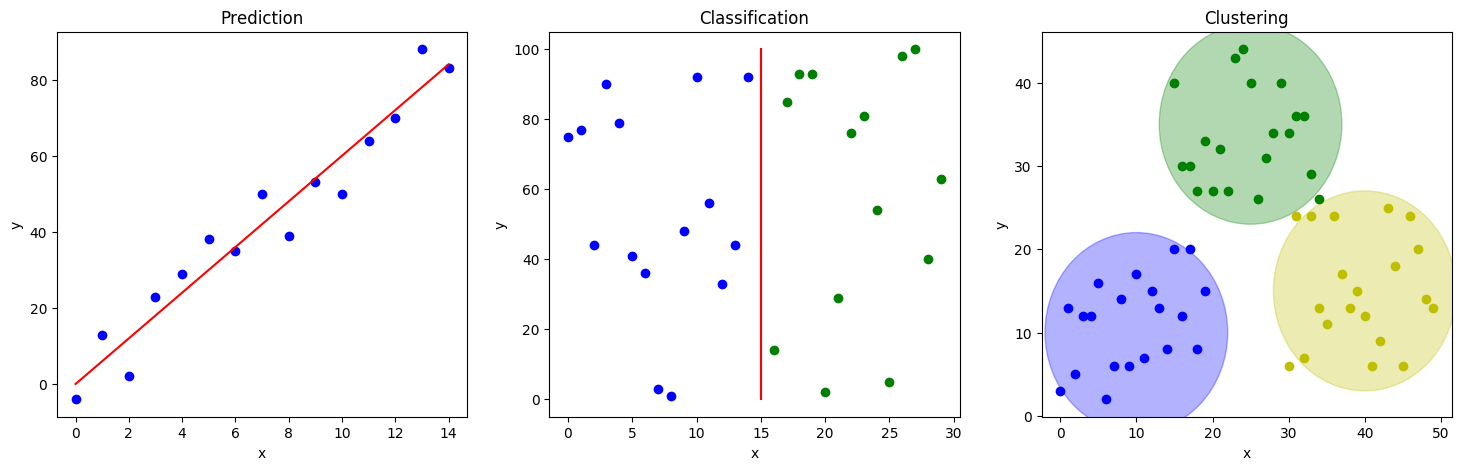
\includegraphics[width=\textwidth]{images/ml_problem_types.png}
	\caption{Arten von \textit{Machine Learning} Problemen (Quelle: Author)}
	\label{fig:ml_problem_types}
\end{figure}


\subsection{Ansätze}
\label{sec:ml_types}

Um ein ML-\textit{Model} anzulernen gibt es verschiedene Möglichkeiten. An eine davon - das Überwachte Lernen - wurde bereits in der Einführung anhand eines Beispiels herangeführt. Dieses Unterkapitel geht auch auf die anderen Möglichkeiten ein.

\subsubsection{Überwachtes Lernen}
Beim Überwachten Lernen (engl. \textit{supervised learning}) wird dem \textit{Model} ein Datenset bestehend aus Datenpunkten und den dazugehörigen korrekten Antwort zu einer Frage übergeben. Der ML-Algorithmus versucht aufgrund den Eigenschaften eines Datenpunktes einen Zusammenhand zu der Antwort zu finden. Wenn daraufhin neue Datenpunkte hinzugefügt werden, kann das \textit{Model} basierend auf den Eigenschaften eine Antwort prognostizieren. Das folgende abstrakte Beispiel demonstriert wie \textit{supervised learning} funktioniert.

Seit der Geburt lernt ein Kind, wie bestimmte Objekte aussehen und wie sie heißen. Es sieht jeden Tag einen Hund in verschiedenen Postionen, mal sitzend, laufend, stehend usw. Dadurch kann es auch den Nachbarshund als solchen identifizieren und zwischen einer Katze unterscheiden. Während der Lernphase kann natürlich auch ein Fehler vorkommen und zum Beispiel einen Wolf als einen Hund misinterpretieren. Doch die Eltern und Geschwister erklären dem Kind, dass es sich dabei nicht um einen Hund handelt. Es passt daher das Verständnis an und wird immer besser das Tier zu identifizieren. Im Kontext von ML ist die oben beschrieben Anwendung zur Erkennung von handgeschriebenen Buchstaben genauso überwachtes Lernen.

\subsubsection{Nicht-Überwachtes Lernen}
Bei dieser Art des Lernens sind im Datenset nicht die korrekten Antworten zu den einzelnen Datenpunkten enthalten. Der Algorithmus ist darauf ausgelegt Trends zu erkennen und Datenpunkte mit Gemeinsamkeiten zu gruppieren ohne zu wissen, worum was es sich dabei handelt. Um auf das oben beschrieben Beispiel mit dem Hund zurück zukommen, werden in einem \textit{Model} viele Bilder von verschiedenen Tieren eingespielt. Die Bilder sind jedoch nicht mit dem darauf enthaltenen Tier markiert. Nachdem der Algorithmus alle Charakteristiken der Bilder analysiert hat ist das \textit{Model} in der Lage, gleichartige Bilder zusammen zufassen. Es kann somit eine Gruppe erstellen, die alle Hunde enthält und eine andere, der alle Katzen zugeordnet sind. Am Ende hat das ML-\textit{Model} noch immer keine Vorstellung, um welches Tier es sich tatsächlich handelt.

Ein anderes Beispiel ist in der Analyse von Kaufverhalten zu finden. Das Datenset besteht hierbei aus den verschiedenen gekauften Produkten der Kunden und das Ziel ist Korrelationen darin zu finden. Das \textit{Model} soll in der Lage sein zum Beispiel folgendes bestimme zu können: Kunden die Schultaschen kaufen, kaufen auch Stifte. Oder Kunden die Bier kaufen, kaufen auch Chips.

\subsubsection{Teil-Überwachtes Lernen}
Teil-Überwachtes Lernen (engl. \textit{semi-supervised learning}) liegt zwischen den beiden vorher beschriebenen Arten des Lernens. Es wird ein Datenset verwendet, dass hauptsächlich aus unmarkierten Datenpunkten besteht. Ein kleiner Teil davon hat jedoch eine Markierung. Im ersten Schritt kommen Techniken zur Gruppierung zum Einsatz, um gleichartige Datenpunkte zu bündeln. Der zweite Schritt besteht darin, die bereits bekannten Datenpunkte dazu zu verwenden, andere Daten in der gleichen Gruppe zu markieren. Einer der größten Vorteile davon ist, dass nicht viel Zeit für das manuelle Markieren von Daten aufgewendet werden muss. Der Nachteil ist aber, dass es im vergleich zum Überwachten Lernen komplexer ist.

Auch hier lässt sich das Beispiel mit den Tieren anwenden. Aus Zeit- oder anderen technischen Gründen können nicht alle Bilder von Hunden und Katzen durchgesehen und markiert werden. Bei ein paar ist es jedoch möglich. Beim Teil-Überwachten Lernen gruppiert zuerst das ML-\textit{Model} alle Bilder mit Hunden und Katzen (gleiche Eigenschaften). Danach können aus den paar Markierten alle anderen abgeleitet werden.

\subsubsection{Bestärkendes Lernen}
Die letzte hier vorgestellte Art ist das Bestärkendes Lernen (engl. \textit{reinforcement learning}). Es kommt einerseits zum Einsatz, wenn sich die Situationen fortlaufend ändern, zum Beispiel beim Autofahren oder bei einem Spiel. Das \textit{Model} muss sich hierbei immer an neue Bedingungen anpassen. Andererseits wird es auch verwendet, wenn ein großer Zustandsraum existiert. Bei beispielsweise Schach ist es kaum möglich mittels \textit{brute-force} den besten nächsten Zug herauszufinden, da es viel zu viele Möglichkeiten im Verlauf eines Spieles gibt. Der Algorithmus ist also darauf ausgelegt eine Entscheidung basierend auf den momentanen internen Zustand und der Umgebung zu treffen, um ein vordefiniertes Ziel zu erreichen. Ein Ziel kann gegebenenfalls sein, ein Auto innerhalb der Spur zu halten. Je länger der Algorithmus lernen kann, desto besser und genauer werden die Entscheidungen in Hinblick auf eine langfristige Auswirkung.

\subsection{Regression}
\label{sec:ml_regression}

Die Regressionsanalyse (engl. \textit{regression analysis}) ist eine auf Statistik basierende \textit{Machine Learning}-Technik, welche aufgrund von oftmals historischen Daten zur Vorhersage verwendet wird. Dabei werden Relationen in markierten Daten analysiert, um eine Prognose für bestimmte Eigenschaften treffen zu können. Zum Beispiel kann damit ein \textit{Model} erstellt werden, welches den aktuellen Preis einer Immobilie bestimmt. Die historischen markierten Daten können hier die Eigenschaften Quadratmeteranzahl, Nachfrage, Lage als Kategorie, Kaufpreis, Verkaufspreis etc. haben. Im Kontext von ML werden die Eigenschaften als \textit{Features} bezeichnet

\section{CAN Bus}
\label{sec:can_bus}

Was ist der CAN Bus?

\subsection{DBC Datei}

was is a dbc datei

\subsection{MDF}

\textit{Measurement Data Format} (MDF) ist ein binäres Dateiformat, welches 1991 von der Firma Vector Informatik GmbH in Zusammenarbeit mit der Robert Bosch GmbH entwickelt wurde. Es ist speziell für Messdaten im Automotive-Bereich konzipiert und ist seit 2009 in der Version 4 als offizieller Standard von \textit{Association for Standardization of Automation and Measuring Systems} (ASAM) öffentlich zugänglich. Ein wesentlicher Vorteil des Formates ist, dass die Messdaten sehr schnell und speicherplatzsparend abgespeichert werden können. Des Weiteren wird auch eine Optimierung des Lesevorgangs durch Vorsortierung und Indizierung unterstützt. Neben den eigentlichen Nutzdaten werden auch Metadaten aus der DBC-Datei mitgespeichert. Dies ist vor allem für weitere Analysen und die Interpretierung der Rohdaten notwendig. Beispielsweise gehören die Information zur Umwandlung in physikalische Werte und Signalnamen dazu. \cite{ASAM14}

\section{Embedded Devices}
\label{sec:embedded_devices}

Vielleicht auch Einführung in Embedded Systems?


% \begin{figure}[htbp]
% 	\centering
% 		
\includegraphics{images/birne}
% 	\caption{Eine Glühbirne}
% 	\label{fig:birne}
% \end{figure}



% \section{Unterkapitel 21}
% \label{sec:Unterkapitel21}

% Textkörper mit Tabelle.

% \begin{table*}[htbp]
% 	\centering
% 		\begin{tabular}{|l|c|r|}
% 		\hline
% 		\rowcolor[gray]{0.9}
% 		Spalte 1 & Spalte 2 & Spalte 3 \\
% 		\hline
% 		Affen & Giraffen & Löwen \\
% 		äpfel & Birnen & Bananen \\
% 		Irgend & et & was \\
% 		\hline
% 		\end{tabular}
% 	\caption{Beispiel für eine Tabelle}
% 	\label{tab:BeispielFuerEineTabelle}
% \end{table*}

% Man beachte die Gegenüberstellung in Tabelle \ref{tab:BeispielFuerEineTabelle}.

% \section{Unterkapitel 23}
% \label{sec:Unterkapite23}

% Aufzählungen:

% Nummeriert:

% \begin{enumerate}
% 	\item Punkt 1
% 	\item Punkt 2
% \end{enumerate}

% Mit Bullet Points:

% \begin{itemize}
% 	\item Punkt 1
% 	\item Punkt 2
% \end{itemize}

% Mit Beschreibungen:

% \begin{description}
% 	\item[Item 1] das ist der 1.Punkt
% 	\item[Item 2] und das der 2.
% \end{description}


% Auch Programmcodes können an entsprechender Stelle eingefügt werden, man beachte dazu auch Listing \ref{lst:conv}.

% % see also http://mirror.easyname.at/ctan/macros/latex/contrib/listings/listings.pdf for options

% \begin{lstlisting}[frame=lines, caption=Simple Listing, captionpos=b, label = lst:conv, language=C, showstringspaces=false]
% #include <stdio.h>
% int main()
% {
% 	int i, n, t1 = 0, t2 = 1, nextTerm;

% 	printf("Enter the number of terms: ");
% 	scanf("%d", &n);

% 	printf("Fibonacci Series: ");

% 	for (i = 1; i <= n; ++i)
% 	{
% 		printf("%d, ", t1);
% 		nextTerm = t1 + t2;
% 		t1 = t2;
% 		t2 = nextTerm;
% 	}
% 	return 0;
% }
% \end{lstlisting}

% Und zuguterletzt, Formeln mitten im Fliesstext, wie z.B. $a^2+b^2=c^2$, in einem Absatz.


%----------------------------------------------------------------
%
%  File    :  set_up.tex
%
%  Authors :  David Lechner, FH Campus Wien, Austria
%
%  Created :  10 Oct 2019
%
%  Changed :  10 Oct 2019
%
%----------------------------------------------------------------


\chapter{Versuchsaufbau}
\label{chap:set_up}

Dieses Kapitel geht auf den Versuchsaufbau des Systems ein. Anfangs werden die zur Verfügung stehenden Daten beschrieben und wie diese für \textit{Machine Learning} vorverarbeitet werden. Danach wird der erste Versuch gezeigt, wie mit ML und den Daten eine Fahreridentifizierung durchgeführt werden kann. Für jegliche Programmieranwendung wurde \textit{Python} aufgrund der zahlreichen Module und des vorhandenen \textit{Know-Hows} verwendet.

\section{Trainingsdaten}
\label{sec:data_description}

Die Daten, welche für die Masterarbeit vorliegen, wurden dankenswerterweise von einem Kollegen bereitgestellt, der diese im Zuge einer Studie über einen längeren Zeitraum aufgezeichnet hat. Dabei handelt es sich um CAN-Nachrichten, aufgenommen in neun Fahrzeugen (VW Golf 7, keine näheren Informationen) während des Fahrens. Es wurde sichergestellt, dass jeweils nur eine Person hinter dem Lenkrad gesessen ist. Ein Boardcomputer mit Internetkonnektivität (ALEN, siehe \ref{sec:ccu}) im Fahrerraum ist für die Aufzeichnung verwendet worden. Das \textit{Embedded-Device} ist über zwei CAN-Bus Schnittstellen mit der Fahrwerks-Linie (F-CAN) und der Komfort-Linie (K-CAN) verbunden und kann somit alle Nachrichten in fast-Echtzeit vom Bus mitlesen. Dabei ist aber sichergestellt, dass es nicht möglich ist, auch Nachrichten senden zu können, da dies bei einer Fehlfunktion zu einem Unfall führen und Insassen gefährden könnte. Die Nachrichten werden nach dem Empfangen mit einem synchronisierten Zeitstempel, aufgelöst in Nanosekunden, versehen und in eine MDF Datei mit den Metadaten von der entsprechenden DBC-Datenbank gespeichert. Eine Datei enthält jeweils Messdaten über eine Dauer von einer Minute. Danach wurde die Datei temporär auf einer Festplatte gespeichert und auf einen File-Server über eine LTE-Funkverbindung hochgeladen. Um sie über alle Fahrzeuge hinweg eindeutig zuordnen zu können, wurde eine Fahrzeugidentifikationsnummer dem Dateinamen angehängt.

In einer Datei sind 46 verschiedene Signale der beiden CAN-Busse enthalten. Tablle \ref{tab:can_signals} listet die meisten davon. Jene, die sich vorrausichtlich nicht für die Analyse eignen, wie z.B. die Innentemperatur oder der Status des Standlichts, sind ausgenommen. Für die komplette Liste siehe Anhang. Pro Datei sind durchschnittlich 100000 Messwerte vorhanden, daraus ergeben sich bei einer Anzahl von 10359 Dateien über eine Milliarde Messpunkte. Die folgende Liste gibt einen Einblick über die vorhandenen Daten.
% TODO: Anhang mit kompletter Liste

\begin{itemize}
  \item Anzahl Fahrer: 9
  \item Datengröße (MDF): 4.9 GB
  \item $\diameter$ Fahrtenanzahl: 46
  \item Fahrtenanzahl insgesamt: 421
  \item $\diameter$ Fahrzeit pro Fahrer pro Fahrt: 23 Minuten
  \item $\diameter$ Fahrzeit pro Fahrer: 18 Stunden
  \item Fahrzeit insgesamt: 165 Stunden
  \item $\diameter$ Gefahrene Kilometer: 1046
  \item Gefahrene Kilometer insgesamt: 9411
  \item Zeitraum: 13.07.2019 - 21.08.2019
  \item Geographischer Bereich: Stuttgart, Deutschland
\end{itemize}

Die Fahrrouten sind nicht speziell beschränkt, sondern sind von Fahrzeug zu Fahrzeug unterschiedlich, was die Fahrtdauer, Tageszeit und Route betrifft. Dadurch sind die Messdaten in sehr realen Bedingungen aufgenommen worden.

\begin{table*}[htbp]
	\centering
  \begin{tabular}{|l|l|l|l|l|}
  \hline
  Signalname & CAN-Bus & Beschreibung & Einheit & Wertbeschr. \\
  \hline
  LWI\_Lenkradwinkel & F-CAN & Lenkradwinkel & Grad & - \\
  LWI\_Lenkradw\_Geschw & F-CAN & \shortstack{Lenkradwinkel- \\ Geschwindigkeit} & Winkelsekunde & - \\
  ESP\_Fahrer\_bremst & F-CAN & Bremspedal betätigt & Boolean & \shortstack{0: nicht betätigt \\ 1: betätigt} \\
  ESP\_Bremsdruck & F-CAN & Bremsdruck & Bar & - \\
  MO\_Fahrpedalrohwert\_01 & F-CAN & Fahrpedalposition & - & - \\
  MO\_Kuppl\_schalter & F-CAN & Kupplung betätigt & Boolean & \shortstack{0: nicht betätigt \\ 1: betätigt} \\
  MO\_Drehzahl\_01 & F-CAN & Motordrehzahl & rpm & - \\
  KBI\_Tankfuellstand\_Prozent & F-CAN & Tankfüllstand & \% & - \\
  KBI\_Kilometerstand & F-CAN & Kilometerstand & km & - \\
  MO\_Gangposition & F-CAN & Gangposition & - & \shortstack{1: 1. Gang oder \\ Rückwärtsgang \\ 2-6: 2. - 6. Gang} \\
  ESP\_VL\_Radgeschw\_02 & F-CAN & \shortstack{Geschwindigkeit \\ Rad links vorne} & km/h & - \\
  ESP\_VR\_Radgeschw\_02 & F-CAN & \shortstack{Geschwindigkeit \\ Rad rechts vornen} & km/h & - \\
  ESP\_HL\_Radgeschw\_02 & F-CAN & \shortstack{Geschwindigkeit \\ Rad links hinten} & km/h & - \\
  ESP\_HR\_Radgeschw\_02 & F-CAN & \shortstack{Geschwindigkeit \\ Rad rechts hinten} & km/h & - \\
  ESP\_v\_Signal & F-CAN & \shortstack{Durchschnittliche \\ Radgeschwindigkeit} & km/h & - \\
  ESP\_HL\_Fahrtrichtung & F-CAN & \shortstack{Fahrtrichtung \\ Rad links hinten} & - & \multirow{2}{*}{\shortstack{0: Vorwärts \\ 1: Rückwärts}} \\
  ESP\_HL\_Fahrtrichtung & F-CAN & \shortstack{Fahrtrichtung \\ Rad links hinten} & - & \\
  ESP\_Laengsbeschl & F-CAN & Längsbeschleunigung & m/s\textsuperscript{2} & - \\
  ESP\_Querbeschleunigung & F-CAN & Querbeschleunigung & m/s\textsuperscript{2} & - \\
  ESP\_Gierrate & F-CAN & Gierrate & \shortstack{Grad pro \\ Sekunde} & - \\
  Wischer\_vorne\_aktiv & K-CAN & Wischer vorne aktiv & Boolean & \multirow{3}{*}{\shortstack{0: nicht aktiv \\ 1: aktiv}} \\
  BH\_Blinker\_li & K-CAN & Blinker links aktiv & Boolean & \\
  BH\_Blinker\_re & K-CAN & Blinker rechts aktiv & Boolean & \\
  \hline
  \end{tabular}
	\caption{Signalbeschreibung}
	\label{tab:can_signals}
\end{table*}

Je nach Steuergerät und Nachrichtentyp ist die Signalhäufigkeit unterschiedlich. Zum Beispiel sendet das Lenkrad- und Motorsteuergerät mit der gleichen Frequenz – nämlich 100-mal in der Sekunde. Andere jedoch, wie das Getriebesteuergerät, nur mit einer Frequenz von 10Hz. Abbildung \ref{fig:signal_freq} zeigt die Häufigkeit einiger Signale. Alle nicht-gelisteten haben entweder eine Frequenz von 10, 50 oder 100Hz.

\begin{figure}[htbp]
	\centering
		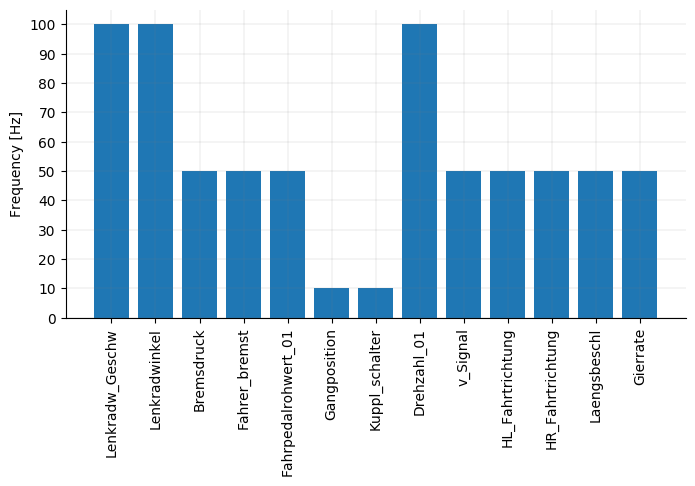
\includegraphics[width=.7\textwidth]{images/signal_frequences.png}
	\caption{Signalhäufigkeiten}
	\label{fig:signal_freq}
\end{figure}

\section{Datenvorbearbeitung}
\label{sec:data_preprocessing}

Werden alle Signale eliminiert, welche nicht unmittelbar vom Fahrer beeinflusst werden und so auch keine Individualität aufweisen, ergibt sich eine Anzahl von 14 verschiedenen Signalen. Das Einschalten des Blinkers oder des Fernlichtes lässt nicht direkt auf den Lenker schließen, da es vielmehr von der Umgebung - Kreuzung oder Einbruch der Dunkelheit - abhängig ist. Die Wahl des Ganges in einer Kurve jedoch schon, siehe Kapitel \ref{sec:overview}. Diese 13 Signale (später auch als \textit{Features} bezeichnet) sind:

\textit{Bremsdruck}, \textit{Gangposition}, \textit{Geschwindigkeit}, \textit{Motordrehzahl}, \textit{Fahrpedalrohwert}, \textit{Längsbeschleunigung}, \textit{Querbeschleunigung}, \textit{Lenkradwinkel}, \textit{Gierrate}, \textit{Bremspedal betätigt}, \textit{Lenkradgeschwindigkeit}, \textit{Kupplung betätigt}, \textit{Fahrtrichtung}

Für jede \textit{Machine Learning} Anwendung ist es ausschlaggebend, dass die Daten durchgängig strukturiert und einheitlich sind. Das Ziel ist also, Datensätze zu bekommen, wo jedes Signal einen Wert hat und einer Fahrerin zugeordnet ist. Da sich die Häufigkeit jedoch unterscheidet, müssen die Signale angeglichen werden, um so eine gemeinsame Frequenz zu bekommen. Laut dem Paper von M. Enev et al. liegt der Wert mit dem besten Endresultat bei 0.5Hz.\footnote{\cite{Enev2016}} Aus allen Signalpunkten wurde daher der Durchschnitt über zwei Sekunden berechnet. Dadurch gehen aber auch Informationen verloren, wie zum Beispiel eine kurze Beschleunigung nach einer Kurve. Um dies zu erhalten, wird auch der Maximal- sowie der Minimalwert mitgenommen. Weiters kommt noch der Median und die Standardabweichung hinzu. Daraus ergibt sich ein Datenset aus 65 Signalen und die Fahreridentifikation. Abbildung \ref{fig:dataset} zeigt einen Auszug der Daten.

\begin{figure}[htbp]
	\centering
		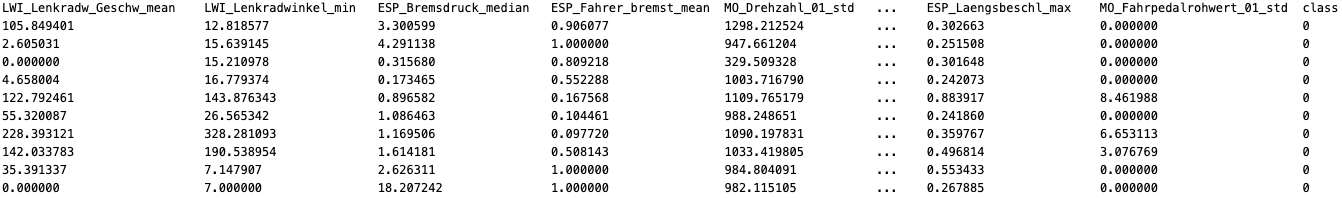
\includegraphics[width=\textwidth]{images/dataset.png}
	\caption{Auszug aus Datenset}
	\label{fig:dataset}
\end{figure}

Für eine einfachere Weiterverarbeitung und etwaige Manipulationen müssen die Daten zwischengespeichert werden. Hierfür bietet sich das Format \textit{Hierarchical Data Format version 5} (HDF5) an, welches der de facto Standard für die Speicherung von großen Datensets in \textit{Python} ist. Es bietet sowohl ein schnelles Einlesen und Schreiben von Daten, als auch die Anwendung von Operationen auf ganze Datenreihen, wie beispielsweise die Berechnung des Durchschnitts oder die Bestimmung der Standardabweichung.\cite{Collete2013}

\section{Scikit-Learn}
\label{sec:sk_learn}

Die Programmiersprache \textit{Python} erfreut sich in den letzten Jahren an einer immer mehr werdenden Popularität. Dank der einfachen Syntax und einer Vielzahl an wissenschaftlichen Bibliotheken ist sie auch besonders für Datenanalyse interessant. Das Modul \textit{Scikit-Learn} \cite{scikit-learn} nützt diese Umgebung und bietet Implementierungen der aktuellsten \textit{Machine Learning} Algorithmen an. Es ist daher eine Antwort auf den wachsenden Bedarf an statistischer Datenanalyse vor allem in nicht wissenschaftlichen Bereichen wie der Software- und Webentwicklung. \textit{Scikit-Learn} gilt als performant und intuitiv, da sie grundlegende Strukturen und Module von \textit{Python} verwendet. Darunter zählen \textit{Numpy}, \textit{Scipy} und \textit{Cython}. Des Weiteren werden auch sehr wenig andere externe Abhängigkeiten benötigt, was zusätzliche Performance bringt.

\section{Erster Versuch}

Als erster Schritt wurde der \textit{Random Forest} Algorithmus mit Standardwerten (siehe weiter unten) auf Messdaten angewendet, um zu validieren, dass eine Identifikation überhaupt mit den vorhanden Daten möglich ist. Hierfür wurden aus den gesamten Daten zufällige 20 Minuten Fahrtzeit pro Fahrer extrahiert, wobei der jeweils erste Datensatz der Beginn einer Fahrt ist. Laut Miro Enev et al. \cite{Enev2016} werden zwischen zehn und 15 Minuten Trainingszeit benötigt, um eine Identifikationsgenauigkeit von über 90\% zu erreichen. Da die Forscher mehr Daten zur Verfügung hatten, wurde die Zeit um fünf Minuten verlängert. Die neun (9 Fahrer) Datensets wurden dann zu einem zusammengefügt, vermischt und in die \textit{Features} beziehungsweise die Fahrerkennung (\textit{class}) aufgeteilt. Daraus sind zufällige sechs Minuten (30\%) entfernt worden, welche später zum Testen des \textit{Models} verwendet werden. Das Listing \ref{lst:rf_first_try} zeigt den Programmcode in \textit{Python}.

\begin{lstlisting}[frame=lines, caption=Erster Versuch mit \textit{Random Forest}, captionpos=b, label = lst:rf_first_try, numbers=left, language=Python, showstringspaces=false, basicstyle=\footnotesize]
import os
import sys
import pandas as pd
from sklearn.utils import shuffle
from sklearn.model_selection import train_test_split
from sklearn.ensemble import RandomForestClassifier
from sklearn import metrics

hdf5_input = sys.argv[1]
signals = ['can0_LWI_Lenkradw_Geschw_mean', 'can0_LWI_Lenkradwinkel_mean', ...]
frames = []
for file in os.listdir(hdf5_input):
  data = pd.read_hdf(os.path.join(hdf5_input, file))
  frames.append(data)

result = pd.concat(frames, sort=False)
result = shuffle(result)
X = result[signals]
Y = result['class']
X_train, X_test, Y_train, Y_test = train_test_split(X, Y, test_size=0.3)

clf = RandomForestClassifier()
clf.fit(X_train, Y_train)
Y_pred = clf.predict(X_test)
accuracy = metrics.accuracy_score(Y_test, Y_pred)

print('Accuracy:' , accuracy)
\end{lstlisting}

Dabei ist eine Identifikationsrate von 85\% Prozent erzielt worden. Das bedeutet, dass das ML-\textit{Model} über 150 Datenreihen aus 180 pro Fahrer ($6[min] * 60 * 0,5Hz = 180$) den tatsächlichen Fahrern zuordnen konnte und bestätigt eine Identifizierung mit den vorhanden Daten. Bei einem erneuten Versuch war die Wahrscheinlichkeit fast 91\% und beim dritten unter 83\%, mit jeweils anderen zufälligen Daten. Die Ergebnisse von weiteren Durchläufen sind in der Abbildung \ref{fig:rf_tries} ersichtlich. Die erste Schlussfolgerung daraus ist, dass eine Identifikation mit den Daten und der Methode möglich ist. Weiters hat die Auswahl der Daten einen erheblichen Einfluss auf das Ergebnis. So war die geringste Wahrscheinlichkeit 78,66\% und die höchste 92,53\%. Im Mittel sind 86,4\% erzielt worden.

\begin{figure}[htbp]
	\centering
		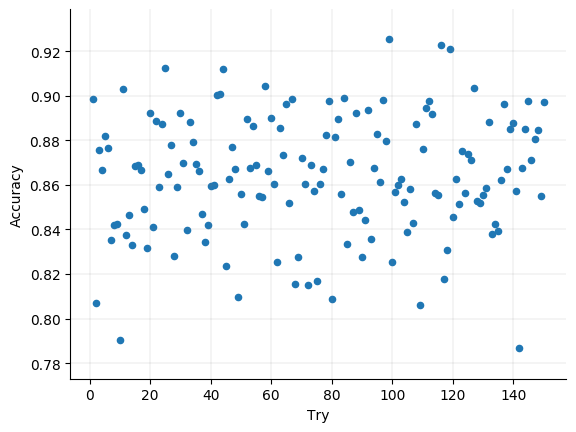
\includegraphics[width=0.7\textwidth]{images/rf_accuracy.png}
	\caption{\textit{Random Forest} Versuche}
	\label{fig:rf_tries}
\end{figure}


%----------------------------------------------------------------
%
%  File    :  optimization.tex
%
%  Authors :  David Lechner, FH Campus Wien, Austria
%
%  Created :  10 Oct 2019
%
%  Changed :  10 Oct 2019
%
%----------------------------------------------------------------


\chapter{Optimierung}
\label{chap:optimization}

Das Kapitel \textit{Optimierung} zeigt wie die Identifikation mit dem verwendeten Algorithmus verbessert werden kann. Es wird einerseits versucht, die Daten zu optimieren, wie zum Beispiel die Anzahl der \textit{Features} oder die Dauer der Trainingszeit. Andererseits wird auch die Methode durch geschickte Parametrisierung verbessert.

\section{Random Forest Parameter-Optimierung}
\label{sec:ml_optimization}

Die \textit{Random Forest} Implementierung von \textit{Scikit-Learn} bietet mehrere Parameter, welche die Trefferquote beeinflussen. Tabelle \ref{tab:rf_parameter} listet diese mit ihren Standardwerten und einer kurzen Beschreibung.

\begin{table*}[htbp]
  \centering
  \caption{\textit{Random Forest} Parameter \cite{sklearn_api}}
  \label{tab:rf_parameter}
  \begin{tabular}{|l|l|l|}
  \hline
  Parameter & Standardwert & Beschreibung\\
  \hline
  criterion & gini & \shortstack{Funktion zur Qualitätsmessung bei der Teilung.\\Mögliche Werte: \\gini: Gini-impurity \\entropy: Informationsgehalt} \\
  min\_samples\_split & 2 & \shortstack{Minimale Anzahl an Daten in einem Blatt,\\bevor es aufgeteilt wird} \\
  min\_samples\_leaf & 1 & Minimale Anzahl an Daten für ein Blatt \\
  max\_depth & None & Baumtiefe \\
  n\_estimators & 100 & Anzahl an \textit{Trees} im \textit{Forest}\\
  \hline
\end{tabular}
\end{table*}

Wie bereits im vorigen Abschnitt gezeigt, steuern die verwendeten Trainings- und Testdaten maßgeblich das \textit{Model}. Die Wahl der Parameter spielt dennoch eine Rolle. Um die Genauigkeit zu verbessern, können die Werte dahingehend angepasst werden. Damit es zu keinen Verfälschungen durch unterschiedliche Daten kommt, wurde jeder Optimierungsversuch sowohl mit denselben Trainings- als auch mit denselben Testdaten durchgeführt. Die Basis bildet daher ein 20-minütiges Datenset pro Fahrer, dessen Genauigkeit mit Standardparameter bei 91,28\% liegt. Zuerst ist jeder Parameter für sich verbessert und die Standardwerte der jeweils anderen herangezogen worden. Es wird nämlich angenommen, dass die Standardwerte bereits ein sehr gutes Ergebnis liefern. Jedoch auch, dass sich die Parameter gegenseitig beeinflussen, sodass die optimalsten Werte nur in Abhängigkeit der anderen bestimmt werden können.

\subsection{criterion}

Der erste Wert, den es zu verbessern gilt, ist \textit{criterion}. Er legt die Funktion fest, wie die Aufteilung bei einem Knoten durchgeführt wird und kann somit entweder \textit{gini} oder \textit{entropy} sein. Abbildung \ref{fig:rf_criterion} zeigt die Auswirkungen. Obwohl laut \cite{Rebala2019} \textit{entropy} für Kategorien besser geeignet ist, kann erkannt werden, dass die durchschnittliche Genauigkeit bei beiden etwa gleich ist. Jedoch fällt die Durchlaufzeit bei \textit{gini} (0.77 Sekunden zu 2.4) wesentlich kürzer aus. Für alle weiteren Optimierungen wurde daher auf Grund des besseren Zeitfaktors nur noch \textit{gini} verwendet.

\begin{figure}[htbp]
	\centering
	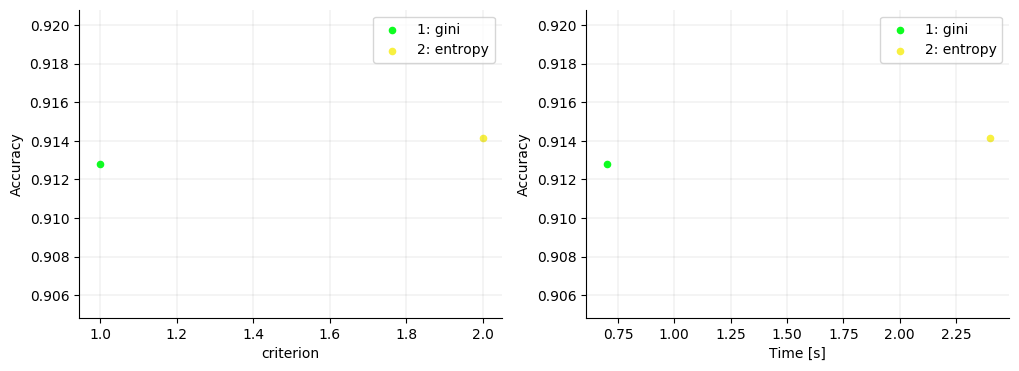
\includegraphics[width=\textwidth]{images/criterion_time.png}
	\caption{\textit{Random Forest} Parameteranalyse \textit{criterion}}
	\label{fig:rf_criterion}
\end{figure}

\subsection{min\_samples\_split}

Als zweites wird der Parameter \textit{min\_samples\_split} analysiert. Dieser bestimmt die mindest Anzahl an Datenpunkten in einem Knoten, welche für das Aufteilen notwendig sind. Auch hier wurden die Standardwerte für die anderen verwendet. Aus der Abbildung \ref{fig:rf_min_samples_split} geht hervor, dass der Parameter das Ergebnis um fast 1 Prozent beeinflusst (90.8 - 91.8\%), wobei die höchste Genauigkeit mit dem Wert \textit{3} erzielt wurde. Weiters ist zu erkennen, dass je höher der Parameter gewählt wird, desto geringer die Trefferquote ausfällt.

\begin{figure}
  \centering
  \begin{subfigure}[c]{0.45\textwidth}
    \centering
    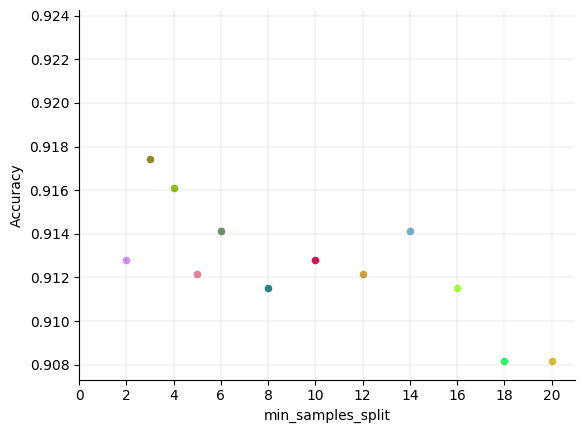
\includegraphics[width=\textwidth]{images/min_samples_split.png}
    \subcaption{\textit{min\_samples\_split}}
    \label{fig:rf_min_samples_split}
  \end{subfigure}
  \hfill
  \begin{subfigure}[c]{0.45\textwidth}
    \centering
    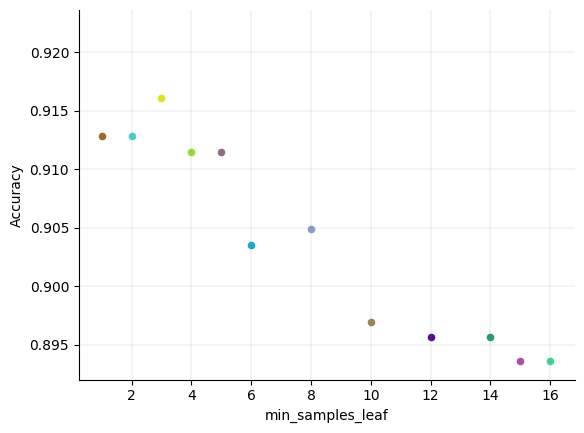
\includegraphics[width=\textwidth]{images/min_samples_leaf.png}
    \subcaption{\textit{min\_samples\_leaf}}
    \label{fig:rf_min_samples_leaf}
  \end{subfigure}
  \caption{\textit{Random Forest} Parameteranalyse}
\end{figure}

\subsection{min\_samples\_leaf}

Der nächste Parameter ist \textit{min\_samples\_leaf} und definiert die minimale Anzahl an Datenpunkten in den \textit{leaf nodes}. Wie die Abbildung \ref{fig:rf_min_samples_leaf} zeigt, nimmt auch hier die Genauigkeit mit ansteigenden Werten ab. Das Maximum liegt bei \textit{3} mit 91.16\%. Der Einfluss auf das ML-\textit{Model} ist etwas höher, da das schlechteste erzielte Ergebnis fast bei 89\% ist.

\subsection{max\_depth}

\textit{max\_depth} beschreibt die Baumtiefe. Ist der Wert auf \textit{undefined} (repräsentiert durch \textit{0} in der Grafik) gesetzt, wird ein Baum soweit expandiert, bis in einem Blatt \textit{min\_samples\_leaf} Datenpunkte erreicht werden. Das beste Resultat wird laut Grafik \ref{fig:rf_max_depth} bei einem Wert von \textit{15} erzielt. Danach fällt es leicht ab und pendelt sich ein.

\begin{figure}[htbp]
	\centering
	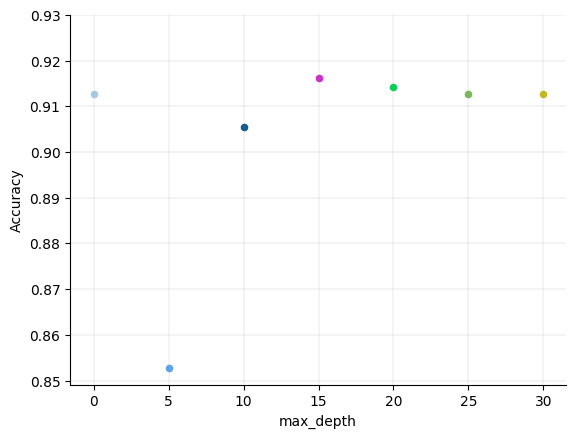
\includegraphics[width=0.5\textwidth]{images/max_depth.png}
	\caption{\textit{Random Forest} Parameteranalyse \textit{max\_depth}}
	\label{fig:rf_max_depth}
\end{figure}

\subsection{n\_estimators}

Die Anzahl der Bäume in einem \textit{Forest} werden durch den Parameter \textit{n\_estimators} spezifiziert. Laut Literatur \cite{Rebala2019}, steigt mit der Erhöhung der Anzahl auch die Genauigkeit des \textit{Models}. Die Abbildung \ref{fig:rf_n_estimators} bestätigt dies. Jedoch steigt auch die Trainings- beziehungsweise die Testzeit, was ebenfalls in der Grafik ersichtlich ist.

\begin{figure}[htbp]
	\centering
	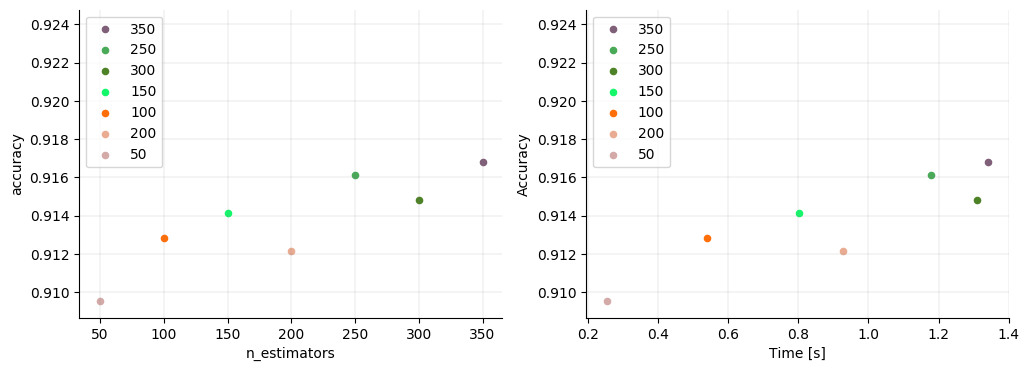
\includegraphics[width=\textwidth]{images/n_estimators.png}
	\caption{\textit{Random Forest} Parameteranalyse \textit{n\_estimators}}
	\label{fig:rf_n_estimators}
\end{figure}

\subsection{Verbesserte Parameter}

Die Tabelle \ref{tab:rf_best_std_parameter} zeigt unter anderem die Zusammenfassung der ersten Analyse. Wird nun das \textit{Model} mit diesen Werten auf die Daten angewendet, ergibt sich eine Genauigkeit von 91.41\%. Das heißt, es konnte lediglich eine Verbesserung um 0.13\% gegenüber den Standardwerten erreicht werden. Dies bestätigt die erste Annahme, dass die Defaultparameter bereits sehr gute Ergebnisse liefern. Weiters kann die Genauigkeit noch verbessert werden, in dem die beste Kombination aller Werte der Parameter gefunden wird. Hierfür müssen 16128 Tests mit dem \textit{Model} durchgeführt werden, was einen hohen Zeit- und Rechenaufwand bedeutet. Dabei ist eine größtmögliche Genauigkeit von 92.21\% herausgekommen, was einer Verbesserung von fast einem Prozentpunkt mit den Daten entspricht. Die Parameterwerte sind ebenfalls in der unten angeführten Tabelle ersichtlich. Gegenüber der ersten Analyse haben sich nicht mehr als zwei Parameter (\textit{min\_samples\_split} und \textit{n\_estimators}) verändert und das auch nur marginal. Für jede fortlaufenden Berechnungen wird diese Kombination verwendet.

\begin{table*}[htbp]
  \centering
  \caption{Verbesserte \textit{Random Forest} Parameter}
  \label{tab:rf_best_std_parameter}
  \begin{tabular}{|l|l|l|l|}
  \hline
  Parameter & Standardwert & Verbesserte Wert (mit Default) & Beste Kombination \\
  \hline
  criterion & gini & gini & gini \\
  min\_samples\_split & 2 & 3 & 3 \\
  min\_samples\_leaf & 1 & 3 & 1 \\
  max\_depth & None & 15 & None \\
  n\_estimators & 100 & 350 & 300 \\
  \hline
  \end{tabular}
\end{table*}

\section{Trainingszeit}

Die Trainingszeit eines ML-\textit{Models} wirkt sich unmittelbar auf die Genauigkeit der Ergebnisse aus. Je mehr Daten anfangs eingespeist werden, desto mehr kann das \textit{Model} lernen und ein genaueres Ergebnis bei neuen Daten liefern. Jedoch steigt auch die Wahrscheinlichkeit, dass die Anzahl an Datenpunkten höher wird, welche ungünstig für diese Anwendung sind. Die Genauigkeit sinkt wiederum dadurch. Laut \cite{Enev2016} und \cite{Ezzini2018} wird bei etwa zehn Minuten Trainingszeit eine Trefferquote von 90\% erzielt. Dies entspricht 300 Datenpunkte pro Fahrer. Die Autoren haben auch gezeigt, dass der allgemeine Fall - mehr Lernen für bessere Ergebnisse - hier nicht zwangsweise zutrifft. Ihre Modelle zeigen nach über 30 Minuten keine Verbesserungen mehr. Da aber auch nicht genau hervorgeht, mit welchen Daten sie zu diesen Erkenntnissen gekommen sind, wird dies versucht nachzustellen und zu validieren. Einerseits mit Daten, welche komplett zufällig aus dem ganzen Datenset mit allen Fahrern gewählt werden und andererseits mit Daten bei den ersten \textit{x} Minuten nach Fahrtbeginn. Dabei ist aber immer die Anzahl an Datenpunkten pro Fahrerin ident. Um eine genauere Aussagekraft der Analysen zu bekommen, wurden die Tests jeweils 50 mal mit unterschiedlichen Daten durchgeführt. Die Ergebnisse sind in den Abbildungen \ref{fig:train_duration_shuffle} und \ref{fig:train_duration_start} ersichtlich. Sie zeigen, dass zwischen zwölf und 18 Minuten an Trainingszeit mit Daten ab einem Fahrtbeginn die beste Trefferquote erzielt werden kann. Ab da an sinkt sie kontinuierlich. Dies deckt sich mit den Aussagen von \cite{Enev2016} und \cite{Ezzini2018}, wenngleich die Genauigkeit nicht konsequent erzielt werden konnte. Werden jedoch rein zufällige Daten für das Modell verwendet, ist erstens die durchschnittliche Genauigkeit (rote Linie) viel geringer, zweitens steigt sie mit der Anzahl der Daten und drittens gibt es weniger Ausreißer nach oben und nach unten je mehr Daten verwendet werden. Das Maximum liegt jedoch auch nur bei knapp über 76\% mit 40 Minuten an Trainingsdaten pro Fahrer. Es ist daher anzunehmen, dass die erwähnten Autoren nicht mit zufälligen Daten aus allen CAN-Signalen gearbeitet haben, sondern mit einem Subset.

\begin{figure}
  \centering
  \begin{subfigure}[c]{0.45\textwidth}
    \centering
    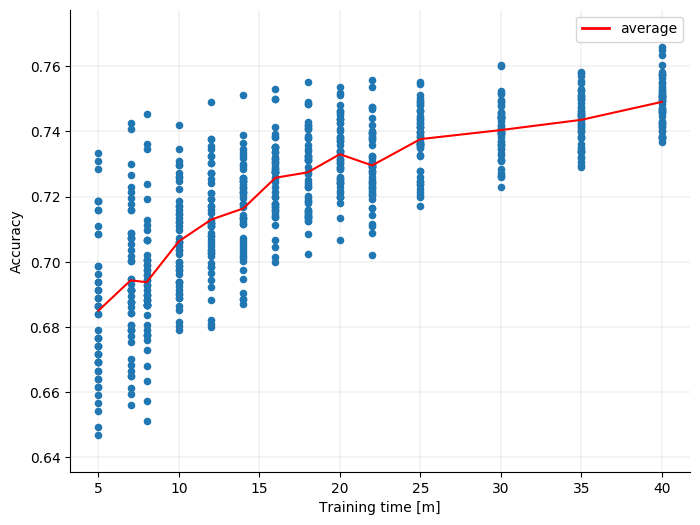
\includegraphics[width=\textwidth]{images/train_duration_shuffle.png}
    \subcaption{Analyse mit zufälligen Daten}
    \label{fig:train_duration_shuffle}
  \end{subfigure}
  \hfill
  \begin{subfigure}[c]{0.45\textwidth}
    \centering
    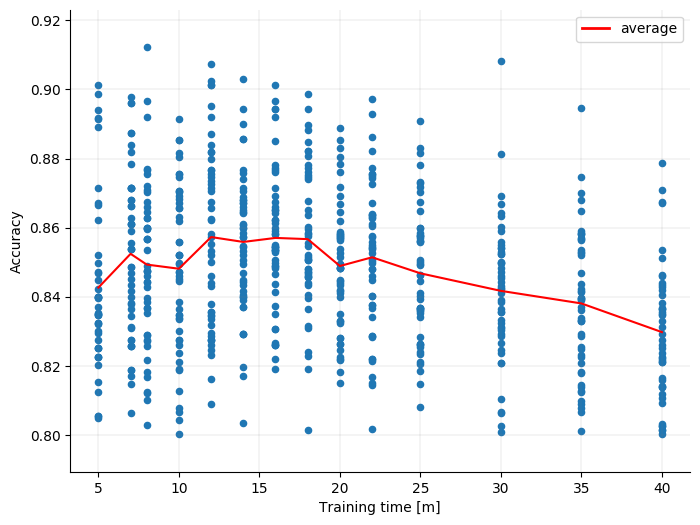
\includegraphics[width=\textwidth]{images/train_duration_start.png}
    \subcaption{Analyse mit Fahrtbeginn}
    \label{fig:train_duration_start}
  \end{subfigure}
  \caption{Analysen der Trainingszeit}
\end{figure}

\section{Feature Optimierung}
\label{sec:feature_optimization}

Eine weitere Möglichkeit das Modell zu optimieren ist, \textit{Features}, welche keine Auswirkung auf die Klassifizierung haben, zu entfernen. Dies spart Rechenleistung, -zeit und könnte unter Umständen auch das Endresultat verbessern. Hierfür gibt es mehrere Möglichkeiten.

\subsection{Feature Korrelationen}

Eine davon beschäftigt sich mit der Korrelation von \textit{Features} \cite{pittir8056}. Dabei wird analysiert, ob es zwischen Merkmalen einen Zusammenhang gibt. Es kann entweder der \textit{Pearson}- oder der \textit{Spearman}-Koeffizient herangezogen werden. Beide können Werte zwischen \textit{-1} und \textit{+1} annehmen. Ersterer kommt bei Daten zum Einsatz, welche sehr stark linear und kontinuierlich sind. Der zweite ist besser, wenn sich die \textit{Features} zusammen verändern, aber nicht unbedingt um den gleichen Faktor. Gibt es streng zusammenhängende Merkmale, können diese (bis auf eines) eliminiert werden. Dadurch reduzieren sich die zu verarbeitenden Daten und das spart Rechenaufwand. Bei den vorhandenen Daten ist anzunehmen, dass die verschiedenen \textit{Features} der einzelnen Signale - Minimal-, Maximal-, Durchschnittswert, Standardabweichung und Median - einen hohen Korrelationswert zueinander haben. Die Abbildung \ref{fig:feature_correlation} belegt dies mithilfe des \textit{Spearman}-Koeffizienten (\textit{+1}, dunkelblau). Daraus ist weiters zu erkennen, dass es einen offensichtlichen Zusammenhang zwischen dem Lenkradwinkel und den verschiedenen Kräften gibt, welche auf das Auto einwirken. Dies gilt ebenso für den Fahrpedalrohwert. Ansonsten können keine zusätzlichen Korrelationen ausgemacht werden.

\begin{figure}[htbp]
  \centering
  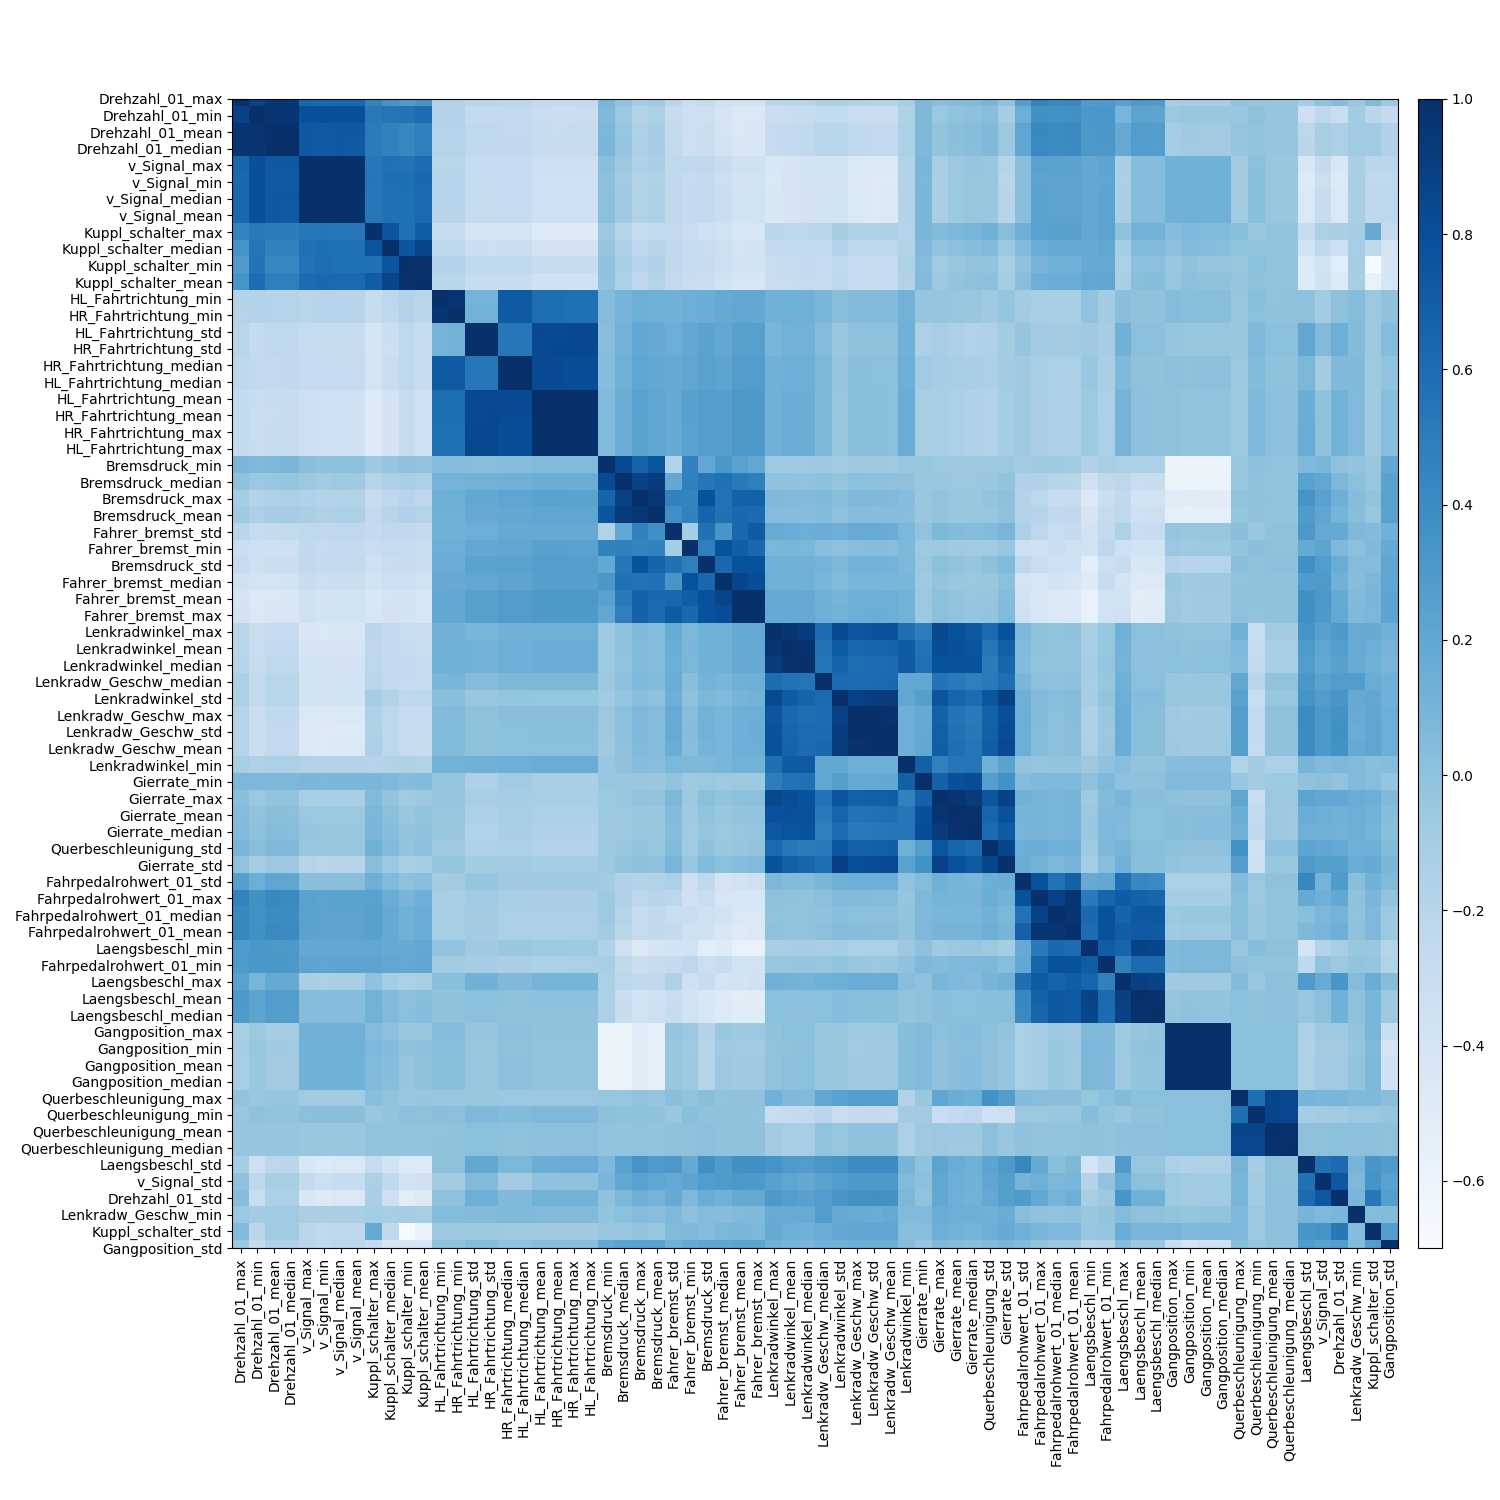
\includegraphics[width=0.9\textwidth]{images/feature_correlation.png}
  \caption{\textit{Feature} Korrelation}
  \label{fig:feature_correlation}
\end{figure}

\subsection{Feature Importance}
\label{sec:feature_importance}

Bevor jedoch einfach die stark korrelierenden \textit{Features} entfernt werden, kann noch eine weitere Analyse durchgeführt werden. Hierbei zeigt sich ein zusätzlicher Vorteil des Algorithmus \textit{Random Forest}. Wie bereits in den Grundlagen erklärt, wird nämlich mithilfe von \textit{Gini Impurity} das wahrscheinlich bestmögliche \textit{Feature} gefunden, um die Daten bei einem Knoten aufzuteilen. Dadurch kann bereits während der Erstellung der verschiedenen \textit{Decision Trees} festegellt werden, welchen Einfluss ein bestimmtes Datenattribut hat. Mit der Implementierung von \textit{Scikit-Learn} können genau diese Werte dargestellt werden. Aus der Abbildung \ref{fig:feature_importance} ist zu entnehmen, dass der Bremsdruck das stärkste Merkmal ist, um eine Fahrerin zu identifizieren. Dies deckt sich auch mit den Ergebnissen von Gahr et al., welche ausschließlich dieses Signal zur Identifizierung verwendet haben. Verwunderlich ist jedoch, dass die reine Gangposition die zweitgrößte Rolle einnimmt. Stellt man die Werte aller Fahrer über die gesamte Fahrzeit dar (siehe Abbildung \ref{fig:gear_position}), kann erkannt werden wieso. Für fünf Fahrer sind nämlich keine korrekten Werte vorhanden. Sie zeigen durchgehend den Gang 14. Dies kann mehrere Gründe haben. Entweder wurde das Aufzeichnungsgerät falsch konfiguriert, das falsche Signal in diesen Autos abgegriffen oder es war schlichtweg nicht vorhanden und 14 ist ein Standardwert. Auch bei den anderen Fahrzeugdaten dürfte ein Fehler unterlaufen sein, da zwischendurch der Gang 13 angezeigt wird. Aus diesem Grund ist für das ML-\textit{Model} die Gangposition so entscheidend. Soll ein neuer Datenpunkt klassifiziert werden, welcher den 14ten Gang enthält, kommen nur noch fünf Fahrer in Frage und dies nur Aufgrund des einen Signals. Es hat jedoch nichts mit dem Individuum hinter dem Lenkrad und dem Fahrverhalten zu tun. Infolge dessen werden dadurch die Ergebnisse des Modells verfälscht und das \textit{Feature} muss daher aus allen vorliegenden Daten entfernt werden. Da es wie erklärt die Trefferquote erhöht hat, geht damit auch ein Performance-Verlust einher. Im vorigen Abschnitt wurde gezeigt, dass mit den Daten eine maximale Genauigkeit von 92\% (durchschnittlich 86\%) erreicht werden konnte. Nach mehreren erneuten Durchläufen ohne der Gangposition konnte nun lediglich 80\% im Mittel und maximal 85\% erzielt werden. Das Modell hat sich demnach um mehr als 5\% verschlechtert, klassifiziert jedoch die Fahrer basierend auf korrekten Fahrzeugdaten.

\begin{figure}
  \centering
  \begin{subfigure}[c]{0.45\textwidth}
    \centering
    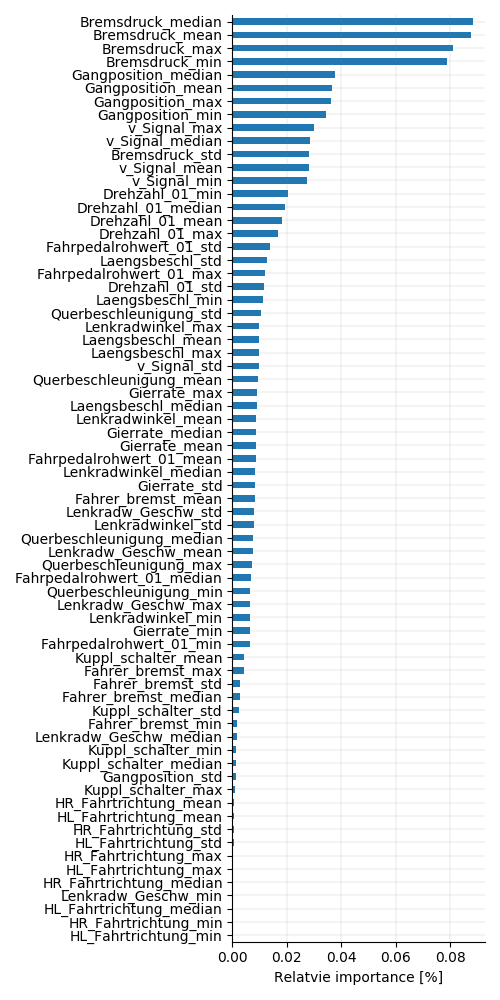
\includegraphics[width=\textwidth]{images/feature_importance.png}
    \subcaption{\textit{Scikit-Learn}s \textit{Feature Importance}}
    \label{fig:feature_importance}
  \end{subfigure}
  \hfill
  \begin{subfigure}[c]{0.45\textwidth}
    \centering
    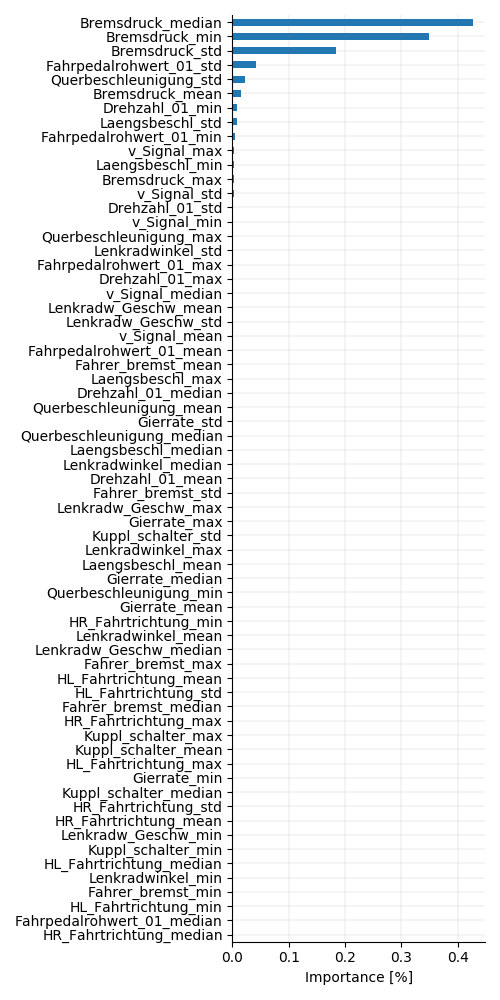
\includegraphics[width=\textwidth]{images/feature_perm_importance.png}
    \subcaption{\textit{Permutation Feature Importance}}
    \label{fig:feature_perm_importance}
  \end{subfigure}
  \caption{\textit{Feature Importance}}
\end{figure}

Des Weiteren zeigt die Grafik \ref{fig:feature_importance}, dass die Geschwindigkeit (\textit{v\_Signal}) und die Motordrehzahl ebenso einen großen Einfluss haben, obwohl eher das Gegenteil anzunehmen ist. Warum die Signale so weit oben angeführt werden hat vermutlich damit zu tun, dass die \textit{Feature}-Auswahl durch das \textit{Gini criterion} verzerrt ist. 2007 haben die Forscher Strobl et al. \cite{Strobl2007} folgendes herausgefunden: Ihre Versuche zeigen, dass \textit{Features} mit mehr potenziellen Aufteilungspunkten ein gutes Kriterium ergeben. Da diese Anzahl exponentiell mit der Anzahl der verschiedenen möglichen Werte steigt, werden solche Merkmale gegenüber welchen mit einer geringeren Varianz von \textit{Decision Trees} eher bevorzugt. Dafür haben sie ein zusätzliches Attribut mit reinen Zufallswerten in die Daten eingefügt. Bei der anschließenden \textit{Feature Importance}-Analyse haben sich diese Daten als besser gegenüber manch anderer echter Daten herausgestellt. Die Zufallswerte hatten dabei eine sehr große Varianz. Für die zwei genannten Signale trifft dies ebenso zu.

\begin{figure}[htbp]
  \centering
  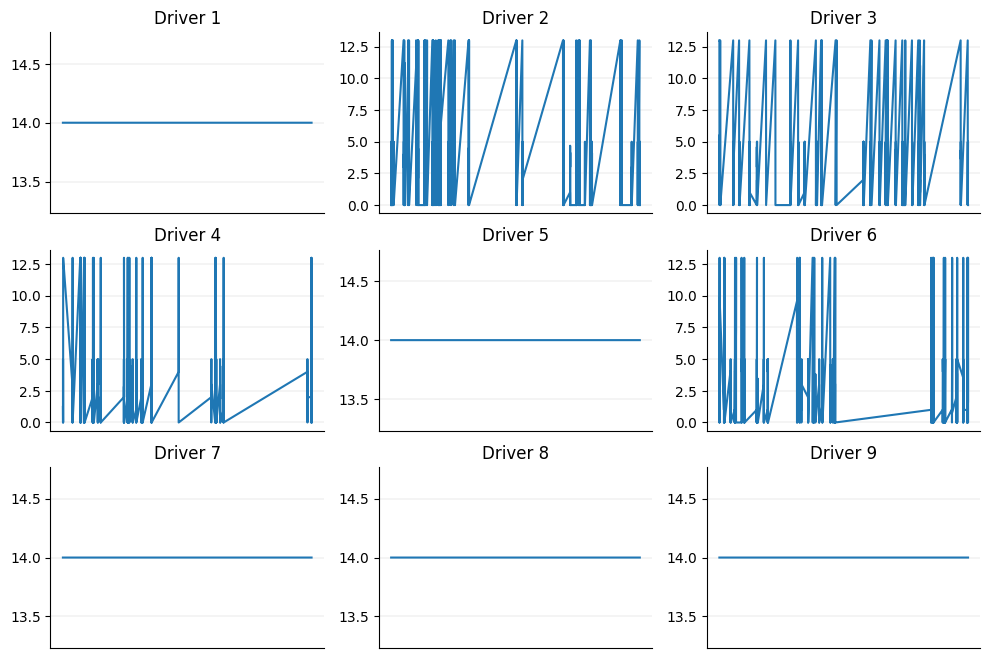
\includegraphics[width=0.7\textwidth]{images/gear_position.png}
  \caption{Gangposition}
  \label{fig:gear_position}
\end{figure}

\subsection{Permutation Importance}
Um diese Verzerrung durch das \textit{Gini criterion} zu umgehen, haben die oben genannten Forscher eine alternative Methode zur Messung der \textit{Feature Importance} vorgestellt \cite{Strobl2007}. Die Idee dahinter ist, herauszufinden, wie sich die Genauigkeit verändert, wenn ein bestimmtes \textit{Feature} nicht mehr existiert. So könnte zum Beispiel bei jedem erneuten Training des Modells eine Datenreihe weggelassen werden. Dies hat aber den Nachteil, dass es sehr Rechenaufwändig ist und nicht unbedingt wiederspiegelt, was in dem gesamten Datenset relevant ist. Einfach das bestimmte \textit{Feature} nur beim Testdurchlauf wegzulassen ist zwar billiger, funktioniert aber nicht, weil die trainierten Entscheidungsbäume alle Datenpunkte einer Reihe erwarten. Anstatt dessen können die echten Werte durch zufälliges Rauschen mit der gleichen Datenverteilung ersetzt werden. Das geht am leichtesten, wenn die Werte des gleichen \textit{Features} permutiert werden. Das Verfahren heißt daher \textit{Permutation Importance} und besteht aus folgenden drei Schritten, wobei Schritt zwei und drei sukzessive wiederholt werden:

\begin{description}
	\item[Schritt 1] Berechne die Genauigkeit des Modells mit allen \textit{Features}.
	\item[Schritt 2] Wähle ein \textit{Feature} aus, permutiere die Werte und berechne die Genauigkeit des Modells erneut.
	\item[Schritt 3] Die Differenz zwischen dem Wert aus Schritt 1 und Schritt 2 ergibt die Wichtigkeit des \textit{Features}.
\end{description}

Mittlerweile ist es als Funktion auch schon in dem \textit{Scikit-Learn} Modul zu finden und kann auf die Daten angewendet werden. Abbildung \ref{fig:feature_perm_importance} zeigt die Ergebnisse daraus. Hier ist zu erkennen, dass der Bremsdruck neuerlich das stärkste Kriterium ist. Das zweit bestbewertete Signal ist der Fahrpedalrohwert. Weiters bestätigt diese Messung die Annahme, dass es bei der ersten Methode eine Verfälschung gegeben hat, da die Geschwindigkeit und die Motordrehzahl weiter unten angeführt werden. Generell haben die meisten Signale eine geringere Auswirkung auf die Genauigkeit des Modells als anfangs gedacht. So sind beispielsweise der Lenkradwinkel, Lenkradbeschleunigung und die Kupplung sehr weit unten in der Tabelle. Das bedeutet aber nicht, dass diese Informationen gänzlich unwichtig für die Klassifizierung sind. Es heißt nur, dass sie für sich alleinstehend keine großen Auswirkungen haben, in Kombination hingegen vielleicht schon.

\subsection{Feature Selection}
\label{sec:feature_selection}

In den letzten zwei Abschnitten wurde die Korrelation zwischen den \textit{Features} gezeigt. Wenn die Eliminierung nach dieser Analyse geht, müssten nahezu $\frac{4}{5}$ der Merkmale wegfallen. Für die korrekte Auswahl kann die \textit{Feature Importance} von \textit{Scikit-Learn} herangezogen werden. Dabei wurden jedoch zwei Widersprüche festgestellt, zum einen die falschen Werte der Gangposition und zum anderen die Verfälschung durch das \textit{Gini criterion}. Mithilfe der Methode \textit{Permutation Importance} konnte dies bereinigt werden und einen möglichst unbeeinflussten Eindruck über die Wichtigkeit der \textit{Features} bekommen. Mit diesen Ergebnissen kann die sogenannte \textit{Feature Selection} durchgeführt werden, bei der die optimale Anzahl an Merkmalen in dem ML-\textit{Model} bestimmt wird. Zu diesem Zweck kann der Algorithmus \textit{Recursive Feature Elimination} (RFE) \cite{Guyon2002} verwendet werden. Als erster Schritt wird das Modell mit allen \textit{Features} trainiert und die Genauigkeit bestimmt. Danach kommt die Methode \textit{Permutation Importance} zum Einsatz, um die Wichtigkeit der Merkmale zu bestimmen. Anhand der resultierenden Reihung wird nach und nach das \textit{Feature} mit der geringsten Auswirkung eliminiert, bis nur noch eines (in diesem Fall \textit{Bremsdruck\_median}) über bleibt. Bei jedem Durchlauf erfolgt das erneute Antrainieren mit dem Subset der Merkmale und die Bestimmung der Genauigkeit. Der gesamte Vorgang wurde mit 100 verschiedenen Trainings- bzw. Testdaten durchgeführt. Werden die Resultate in einer Grafik visualisiert (siehe Abbildung \ref{fig:feature_selection}), kann erkannt werden, wie viele \textit{Features} für eine gewisse Trefferquote benötigt werden. So gibt es zwischen den ersten zehn Merkmale eine deutliche Steigerung und ab dem elften flacht sie ab. Ein sehr guter Wert kann mit 21 der verfügbaren 65 \textit{Features} erzielt werden.

\begin{figure}[htbp]
  \centering
  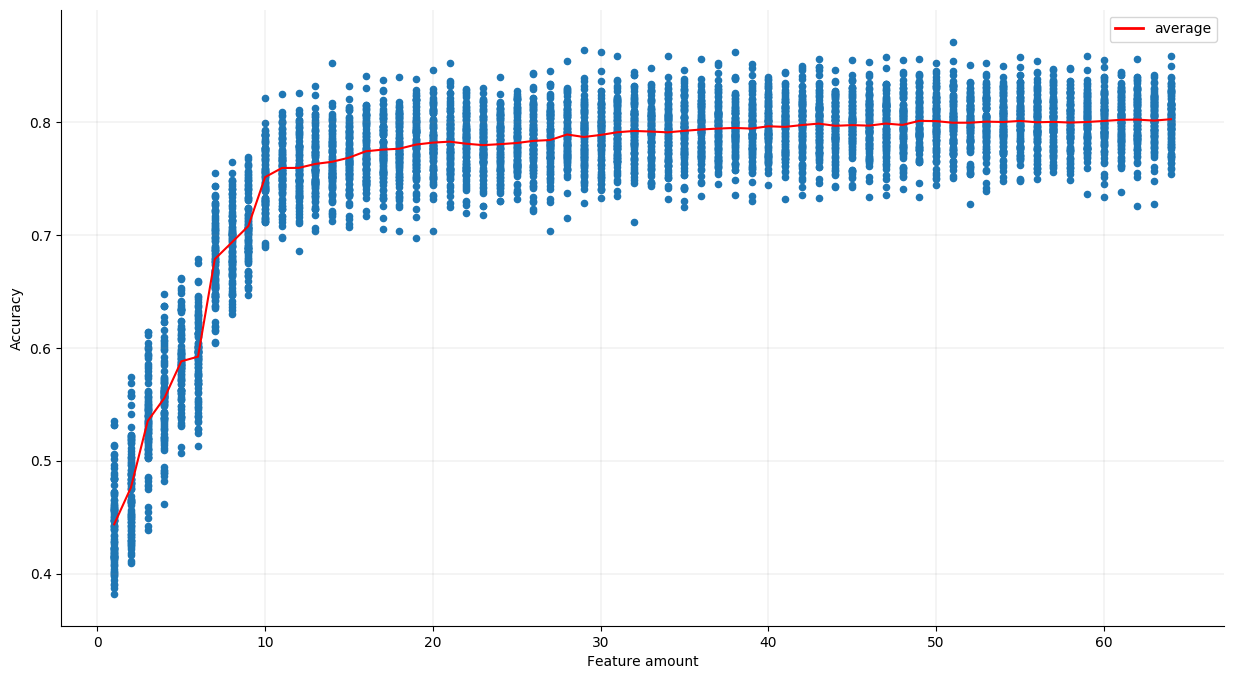
\includegraphics[width=0.8\textwidth]{images/feature_selection.png}
  \caption{\textit{Feature} Auswahl}
  \label{fig:feature_selection}
\end{figure}

%----------------------------------------------------------------
%
%  File    :  integration.tex
%
%  Authors :  David Lechner, FH Campus Wien, Austria
%
%  Created :  10 March 2020
%
%  Changed :  10 March 2020
%
%----------------------------------------------------------------


\chapter{Integration ins Fahrzeug}
\label{chap:car_integration}

In diesem Kapitel wird gezeigt, wie das System zur Erkennung des Lenkers prototypisch in ein Fahrzeug integriert werden kann. Die Anwendung soll insbesondere folgende Aufgabe erfüllen:

\begin{description}
    \item[] Aus einem Set von vier bekannten Fahrerprofilen soll die aktuell fahrende Person zugeordnet werden können.
\end{description}

Laut Statistik Austria hat die durchschnittliche österreichische Familie 1,68 Kinder (Stand 2018) \cite{Stat2018}. Aufgerundet besteht sie daher aus vier Personen und deshalb die Anzahl der Fahrerprofile.

Die Anforderung zielt speziell auf konkrete Anwendungsfälle, welche zum Teil bereits in der Einleitung erläutert wurden, ab. Mit den Erkenntnissen lassen sich Maßnahmen umsetzten, um beispielsweise mehr Komfort bieten zu können. Darunter fällt das Einstellen des bevorzugten Radiosenders oder das Anzeigen der letzten Ziele im Navigationssystem für eine schnellere Auswahl. Andere Möglichkeiten, wie diese Information genutzt werden kann, werden weiters noch im nächsten Kapitel diskutiert.

\section{Systemarchitektur}
\label{sec:architecture}

Das Gesamtsystem kann mit zwei verschiedenen Architekturen umgesetzt werden. Bei beiden Varianten gibt es vier Komponenten. Ausgangspunkt sind die Steuergeräte, die in einem Fahrzeug über den CAN-Bus vernetzt sind. Eine zentrale Logikeinheit, die \textit{Car Connectivity Unit} (CCU), zeichnet die CAN-Nachrichten auf und verarbeitet diese. Sie ist nicht Teil eines Serienfahrzeuges und muss nachgerüstet werden. Beim ersten Ansatz überträgt die CCU alle CAN-Daten zu einem \textit{Cloud}-Service, wo sie von einem bereits trainierten \textit{Machine Learning Model} klassifiziert werden. Aufgrund dessen liegen die Profile der autorisierten Lenker eines Fahrzeugs auch in der \textit{Cloud}. Das Ergebnis um welche Fahrerin es sich handelt, wird entweder über einen Email- oder SMS-Provider zurück ins Auto oder zum Fahrzeughalter gesendet. Beim zweiten Ansatz wird alles auf der CCU durchgeführt. Sie trainiert ein Model mit den Fahrerprofilen, liest CAN-Nachrichten mit, führt die Klassifizierung durch und versendet das Ergebnis. Die Abbildungen \ref{fig:arch1} und \ref{fig:arch2} bilden die Ansätze ab.

\begin{figure}
    \centering
    \begin{subfigure}[c]{0.48\textwidth}
        \centering
        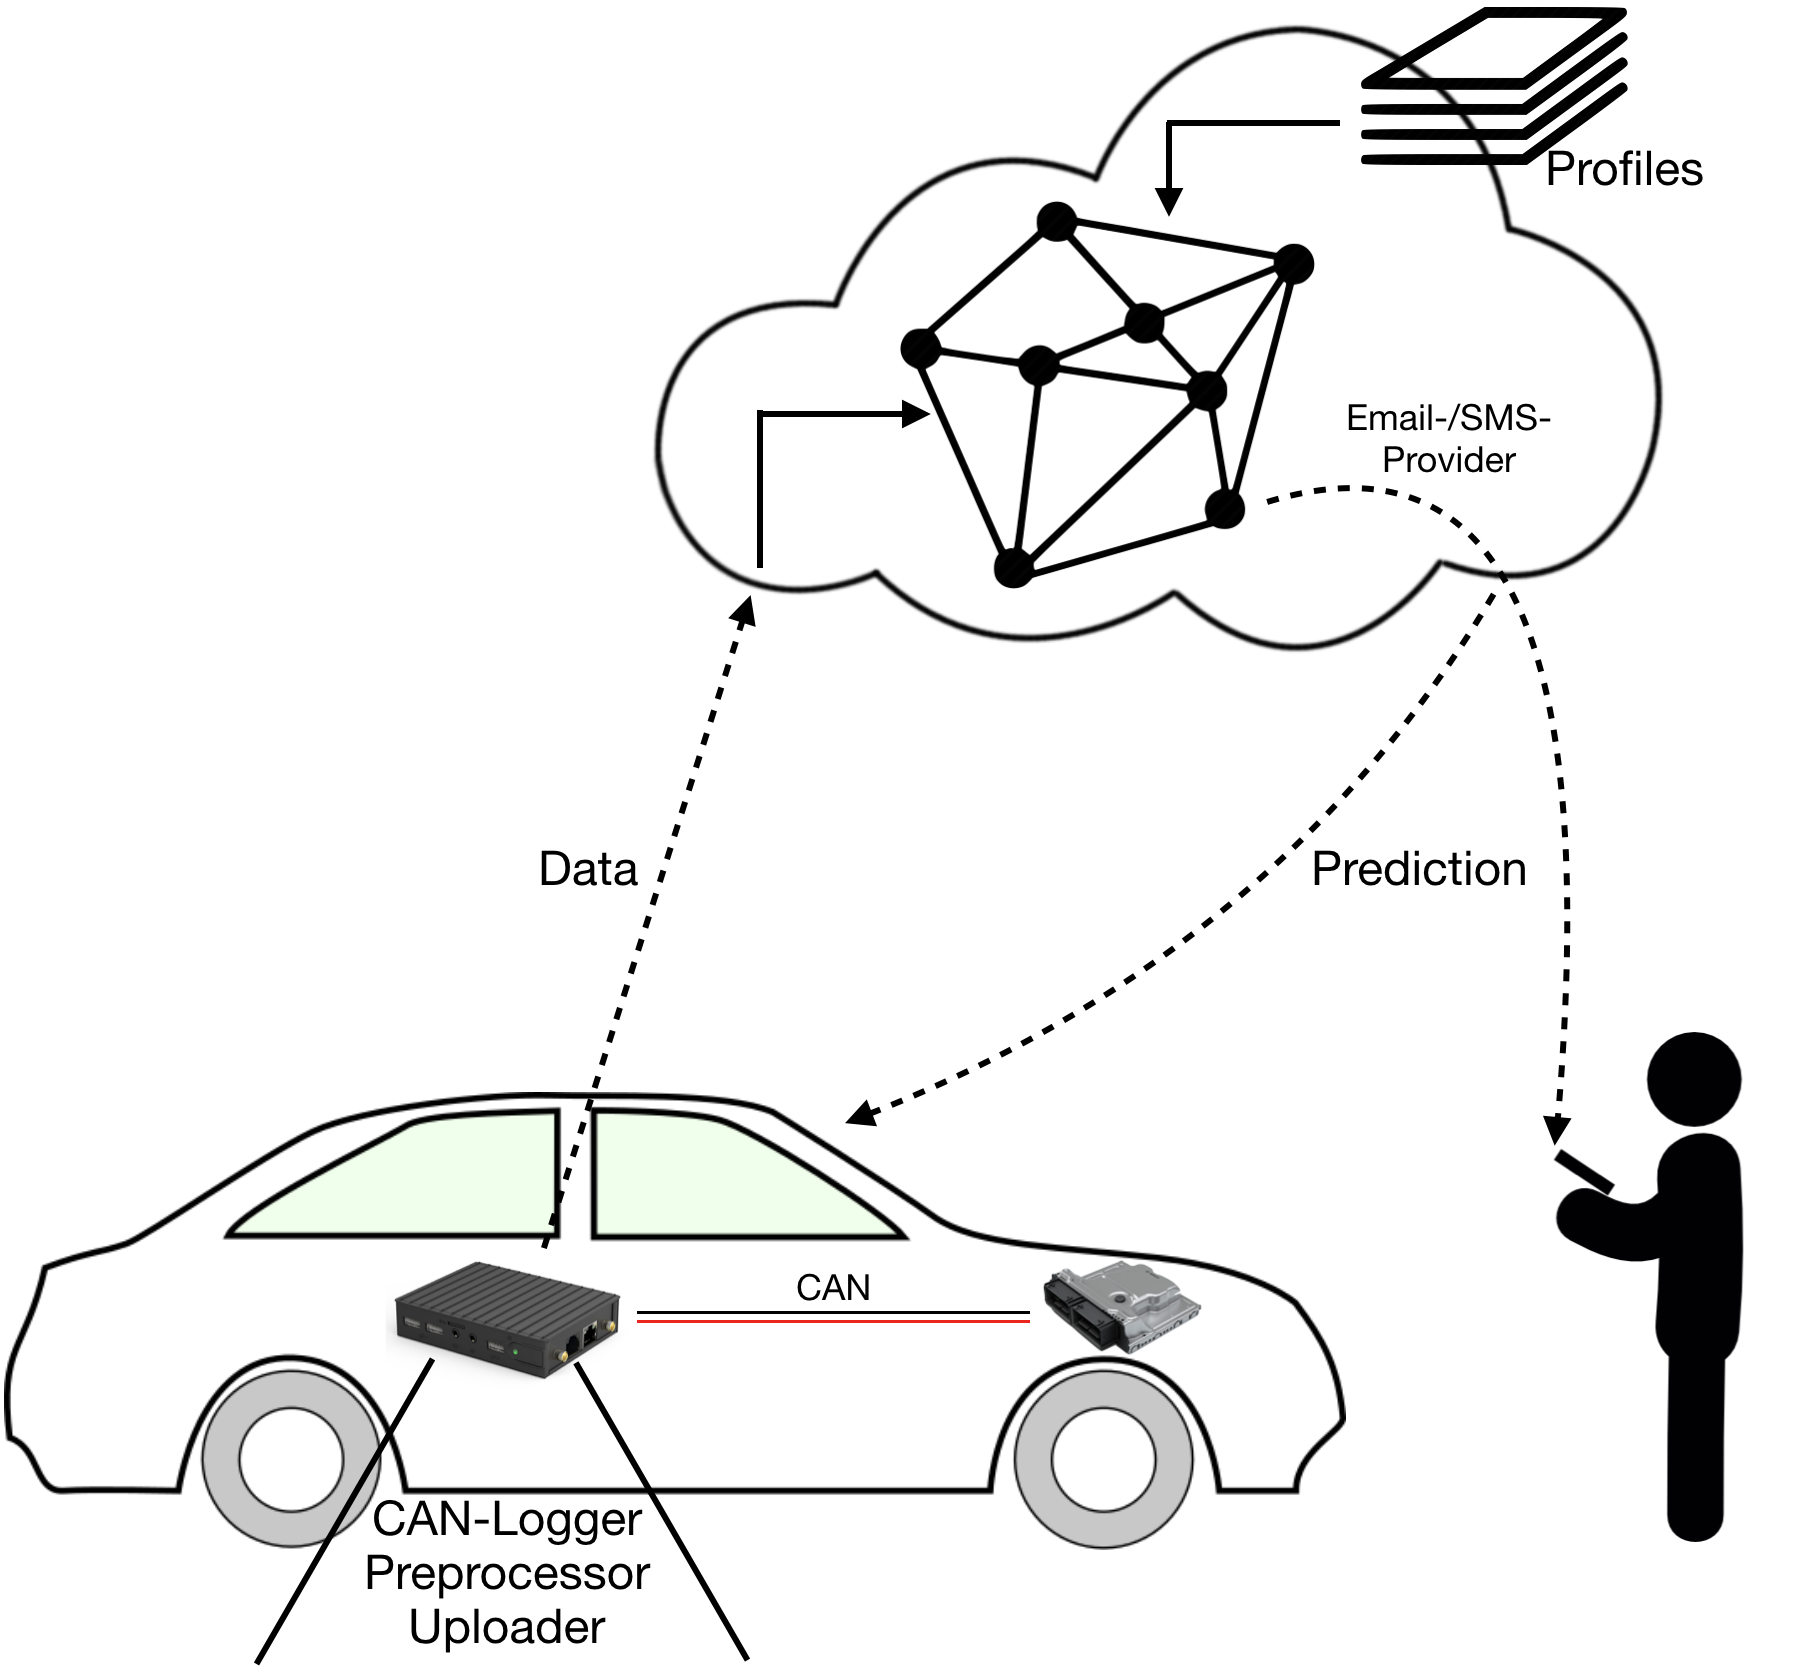
\includegraphics[width=\textwidth]{images/arch_type1.png}
        \subcaption{Architektur 1}
        \label{fig:arch1}
    \end{subfigure}
    \hfill
    \begin{subfigure}[c]{0.48\textwidth}
        \centering
        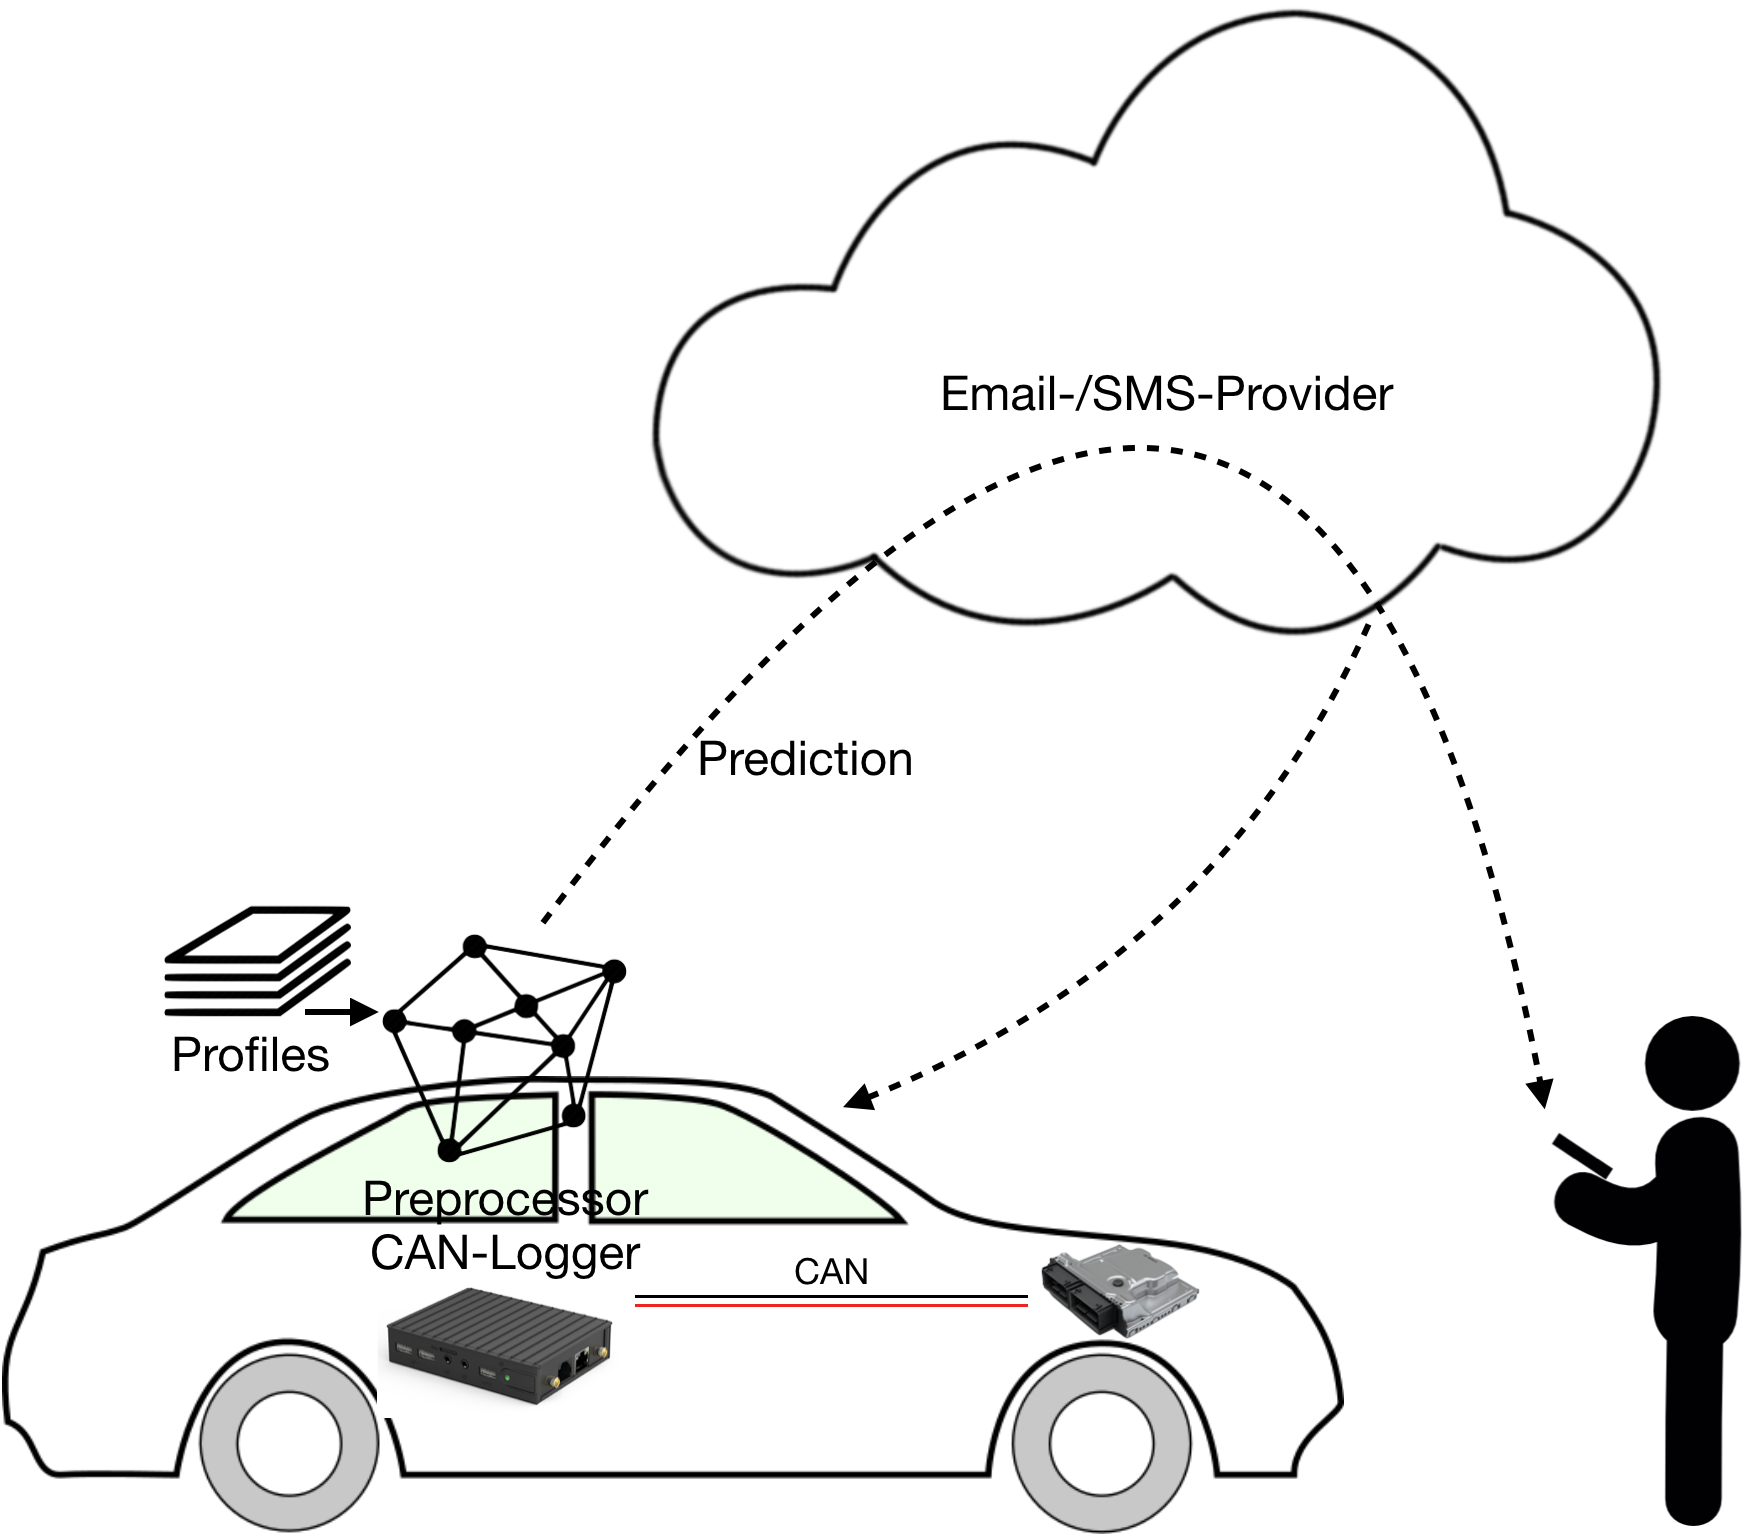
\includegraphics[width=\textwidth]{images/arch_type2.png}
        \subcaption{Architektur 2}
        \label{fig:arch2}
    \end{subfigure}
    \caption{Mögliche Architekturen}
\end{figure}

Der Hauptunterschied bei beiden liegt darin, wo jegliche \textit{Machine Learning} Anwendungen laufen. Dies zieht jedoch eine Reihe von Konsequenzen mit sich. In erster Linie wird dem System Komplexität genommen, wenn Komponenten wegfallen. In diesem Fall ist es das ML-\textit{Cloud}-Service. Die CCU muss im zweiten Ansatz keine Verbindung in die \textit{Cloud} aufbauen und Daten übertragen. Da es sich dabei mitunter um sensible Daten handelt, fallen zudem alle Anforderungen bezüglich CIA - \textit{Confidentiality}, \textit{Integrity}, \textit{Authenticity} - weg. Der Kommunikationskanal müsste sonst gegen ein unerlaubtes Abgreifen der Daten verschlüsselt, gegen eine Verfälschung integritätsgeschützt und authentifiziert sein, damit potentielle Angreifer keine Daten einspeisen können. Die ersten beiden Kriterien können einfach mit dem Einsatz von \textit{HTTPS} sichergestellt werden. Hierzu muss lediglich ein entsprechendes Zertifikat am Server installiert sein, welches für den Daten-Upload verwendet wird. Für die Gewährleistung der Authentizität können zum Beispiel Client-Zertifikate eingesetzt werden. Dafür ist eine eigene \textit{Public Key Infrastructure} (PKI) nötig, um die Zertifikate auf den CCUs zu verwalten.

Ein weiterer Nachteil des zweiten Ansatzes ist, dass Übertragungs- und Verbindungsabbrüche korrekt behandelt werden müssen. Dazu zählt die Verifizierung eines erfolgreichen Uploads, die Wiederaufnahme eines Abbruchs und die Sicherstellung, dass nichts mehrfach hochgeladen wird. Nicht nur die Kommunikation zwischen der \textit{Connectivity Unit} und der \textit{Cloud} erfordert Maßnahmen gegen \textit{Security Threats}, sondern auch die \textit{Cloud} an sich. Sie muss mit einer \textit{Firewall} abgesichert, ein unerlaubter Austausch und Verfälschung der Profile verhindert werden. Wie bereits in den Grundlagen \ref{sec:edge_computing} \textit{Edge Computing} erläutert, hat die Wahl der Architektur auch eine Auswirkung auf den Datenschutz. Bleiben die Daten nur offline am Gerät, muss deutlich weniger beachtet werden, als wenn sie in die \textit{Cloud} hochgeladen werden.

Der zweite Ansatz hat aber auch Nachteile. So ist beispielsweise die Verteilung von Updates schwieriger, da diese auf jeder CCU eingespielt werden müssen und nicht nur zentral in der \textit{Cloud}. Es könnte mitunter auch zu Performance-Problemen kommen, falls das \textit{Embedded-Device} zu wenig Ressourcen für \textit{Machine Learning} Anwendungen hat. Im Ansatz 1 kann durch eine einfache und schnelle Skalierung der CPUs/GPUs beziehungsweise des Arbeitsspeichers der IaaS-Provider die Leistung an die Anforderungen angepasst werden. Auch die Administration der Fahrerprofile wie zum Beispiel das Hinzufügen oder Löschen lässt sich einfacher gestalten, wenn sie auf der \textit{Cloud} abliegen. Es gibt noch mehr Punkte, welche in die Entscheidung der zu implementierenden Architektur miteinfließen. Darunter fällt das Logging, Monitoring, erweitertes \textit{Security}-Konzept oder wie das gesamte System auf viele Fahrzeuge skaliert werden kann. Da es jedoch nur prototypisch für ein einziges Auto realisiert wird, werden diese Punkte nicht näher erläutert.

Der zweite Ansatz ist aufgrund der überwiegenden Vorteile, vor allem weil die Komplexität durch die Kommunikation mit der \textit{Cloud} wegfällt, zu bevorzugen und wird daher in weiterer Folge umgesetzt.

\section{Car Connectivity Unit}
\label{sec:ccu}

Der zentrale Baustein des Systems zur Identifizierung eines Fahrers ist die \textit{Car Connectivity Unit}, welche im Auto verbaut wird. In der Architekturbeschreibung wurde schon auf ihre Funktionen hingewiesen. Daraus lassen sich folgende Hardware-Anforderungen für das Device extrahieren:

\begin{itemize}
    \item kompakte Bauweise für das automotiv Umfeld
    \item CAN-Interface
    \item ausreichend Ressourcen für \textit{Machine Learning} Anwendungen
    \item LTE Modem
    \item Debug/Flash Schnittstelle
\end{itemize}

Prinzipiell könnte ein \textit{Raspberry-Pi} mit entsprechenden Modulen und einem robusten Gehäuse in Frage kommen. Da jedoch das Unternehmen \textit{Bosch} eine Reihe an dezidierten CCUs im Portfolio hat und bei einer schon viel Know-How vorhanden ist, wird die sogenannte \textit{Automotive Linux Edge Node} (ALEN) eingesetzt. Ursprünglich ist das israelische Unternehmen \textit{CompuLab} \footnote{\url{https://www.compulab.com/products/iot-gateways/}} der Hersteller des Geräts und \textit{Bosch} passt es an Automotive-Bedingungen an. Darunter fällt die Verstärkung des Gehäuses, das Hinzufügen einer CAN-Schnittstelle (RJ11-Buchse) sowie der Austausch des LTE-Moduls. Des Weiteren verfügt die ALEN über vier USB-Ports, eine serielle Schnittstelle über Micro-USB, ein WiFi Modul, zwei Gigabit Ethernet-Buchsen, jeweils einen Audio Ein- und Ausgang sowie einen HDMI-Ausgang. Hinzu kommen noch einige GPIOS, I2C, UART und SPI Interfaces. Als Prozessor ist ein 1GHz NXP i.MX 7Dual ARM Cortex-A7 verbaut, 1GB RAM sowie ein 12GB Flash-Speicher. Die Versorgungsspannung beträgt 12V. Die Abbildungen \ref{fig:alen} zeigt die CCU.

\begin{figure}[htbp]
	\centering
    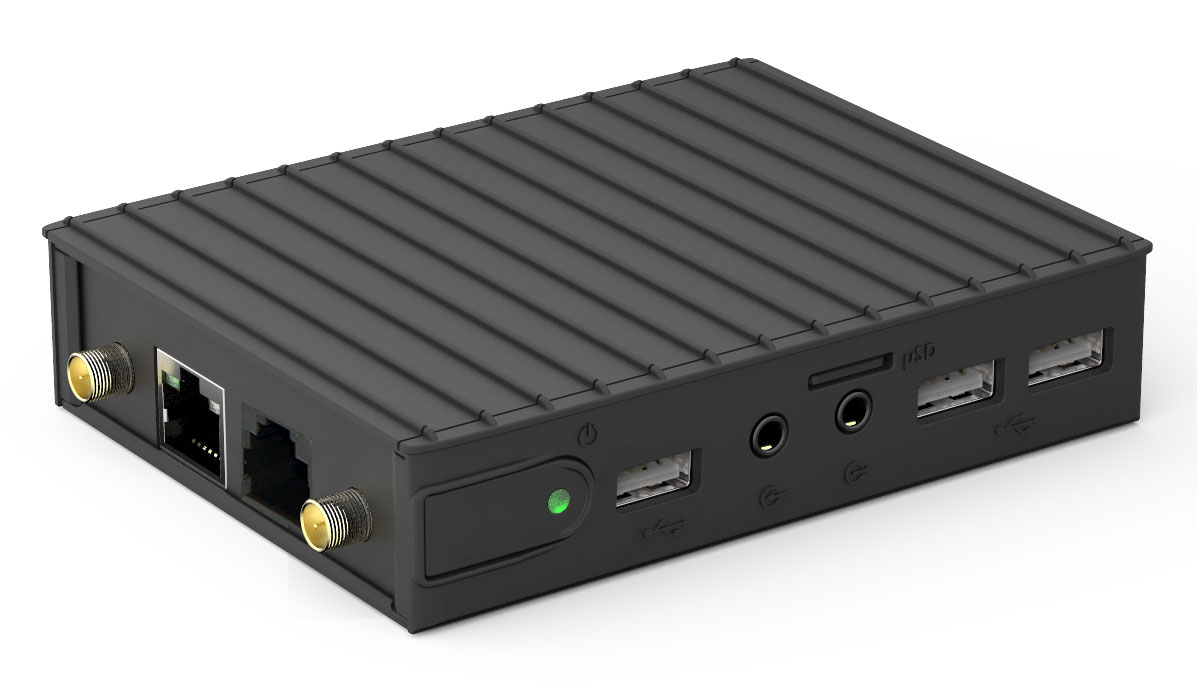
\includegraphics[width=.5\textwidth]{images/alen.jpg}
	\caption{\textit{Automotive Linux Edge Node} (ALEN, Quelle: \url{https://www.compulab.com/products/iot-gateways/})}
	\label{fig:alen}
\end{figure}

Auf der ALEN läuft ein individuelles Linux-System, welches für die Hardware angepasst und mithilfe einer SD-Karte auf das Gerät geladen wird. Zum Erstellen dieser speziellen Linux Distribution wird \textit{Yocto} verwendet.

\subsection{Yocto}
\label{sec:yocto}

\textit{Yocto} \cite{Yocto20} ist ein \textit{Open-Source} Projekt bestehend aus verschiedenen \textit{Templates}, \textit{Tools} und Methoden, um ein Linux-basiertes Betriebssystem für eingebettete Systeme zu bauen. Es wurde 2010 von der \textit{Linux Foundation} ins Leben gerufen und wird seither auch von ihr verwaltet. Die drei Hauptkomponenten sind \textit{BitBake}, \textit{OpenEmbedded-Core} und \textit{Poky}. Ersteres ist die \textit{Build Engine}, ähnlich wie \textit{make} für \textit{C}. Sie interpretiert Konfigurationsdateien und \textit{Recipes} (siehe weiter unten) und führt davon ausgehend Aktionen aus, beispielsweise herunterladen von \textit{Source-Code} oder Binärdateien, konfigurieren und bauen von Applikationen sowie das Dateisystem. Die zweite Komponente ist eine Sammlung aus Basis-\textit{Layer} für einige Hardwarearchitekturen wie zum Beispiel ARM oder MIPS. \textit{Poky} ist sozusagen der Grundstein für jegliches Betriebssystem und vereint alles was dafür benötigt wird.

Jedes \textit{Yocto} Projekt besteht aus mehreren Schichten (\textit{Layer}), wobei die erste eben \textit{Poky} ist. Diese bringt auch den Linux-Kernel mit ein. Die zweite Schicht beinhaltet alle Informationen für die zu verwendete Hardware und wird auch das \textit{Board Support Package} (BSP) genannt. Darunter zählen die Kernel-Konfigurationen, der \textit{Device-Tree} und Treiber. Für die ALEN stellt der Hersteller \textit{Compulab} diese Schicht bereit. Die darüber liegenden \textit{Layer} können weitere Spezifikationen und Modifikationen für das BSP enthalten, wenn z.B. sich die Peripherie geändert hat. Eine Regel der \textit{Yocto-Community} besagt nämlich, dass niemals Basisschichten direkt verändert werden dürfen, sondern nur durch höhere. Dazwischen können noch weitere Schichten liegen, eventuell eine \textit{Security}-Schicht, welche \textit{Recipes} und Konfigurationen für einen sicheren Update-Mechanismus oder \textit{SSH} umfasst. Die letzte Schicht wird dazu verwendet, um Anwender-Software hinzuzufügen, Benutzer anzulegen oder Konfigurationen für Dienste zu ändern.

All diese \textit{Layer} enthalten die angesprochenen \textit{Recipes}, welche Tasks spezifizieren, die wiederum von \textit{BitBake} ausgeführt werden. Im Allgemeinen handelt es sich dabei um Informationen über eine einzelne Applikation. Diese inkludieren meistens den Ort von wo der \textit{Source-Code} bezogen wird (z.B. \textit{GitHub}), spezielle Einstellungen, wie kompiliert wird und wohin die resultierenden Dateien im Zielsystem gespeichert werden. Des Weiteren können auch \textit{Patches} vorhanden sein, die andere \textit{Recipes} anpassen. Sie sind notwendig, wenn ein Pfad geändert werden muss, Kernel-Configs oder neue Dateien hinzukommen. Wird nun über die \textit{Build Engine} ein \textit{Image} gebaut, werden alle \textit{Recipes} nach der Reihe bzw. parallel ausgeführt. Das Ergebnis ist das gesamte \textit{Root-Filesystem} und alle Informationen die für das Booten des Geräts benötigt werden.

Das ist zugleich ein großer Vorteil von \textit{Yocto} \cite{Yocto220}. Beim traditionellen Aufsetzen eines Linux-basierten Systems wird ein standard Betriebssystem installiert und im Nachhinein konfiguriert, neue Softwarepakete installiert usw. Hierbei ist das Zielsystem bereits voll eingerichtet und erfordert keine weiteren Aktionen für den gewünschten Betrieb. Zudem gibt es eine große \textit{Community} rund um \textit{Yocto}, die einerseits das Projekt stets voranbringt und andererseits viel Support bei Problemen liefert. Ein Vorteil ist auch, dass die erforderliche \textit{Toolchain} zum Entwickeln voll enthalten ist und leicht an eigene Bedürfnisse angepasst werden kann. Zusätzlich bietet das \textit{Layer}-Modell Flexibilität und Wiederverwendung der einzelnen Schichten. Soll ein System auf eine andere Hardware portiert werden, braucht nur das \textit{Board Support Package} ausgetauscht werden. Durch die Komplexität ergibt sich unweigerlich eine große Einstiegshürde. Die Lernkurve ist anfangs sehr steil und initial muss viel Zeit aufgewendet werden, um alles Notwendige einsatzfähig zu haben. Nichtsdestotrotz ist \textit{Yocto} bei der Erstellung von hardwareabhängigen Betriebssystemen für \textit{Embeded Systems} und vor allem auch für den IoT Bereich sehr beliebt.

Die unten angeführte Abbildung zeigt die \textit{Layer} für dieses Projekt. Hier ist anzumerken, dass die Namenskonvention den Präfix \textit{meta-} für die \textit{Layer} vorschreibt. Die ersten zwei Schichten bilden die Basis mit dem Linux-Kernel. \textit{Freescale} bringt die für NXP wesentlichen Konfigurationen für die CPU ein. Die vierte Schicht installiert \textit{Python} in das \textit{Image} und \textit{meta-alen} enthält alle Informationen speziell für die Hardware, welche von \textit{Compulab} und \textit{Bosch} kommen. Die letzte Schicht inkludiert die zusätzlichen Module für \textit{Python}, etwa \textit{Scikit-Learn} und \textit{Pandas}, sowie die Applikationen zum Aufzeichnen des CAN-Busses und für \textit{Machine Learning}. In den nächsten Abschnitten wird auf die Software näher eingegangen.

\begin{figure}[htbp]
	\centering
    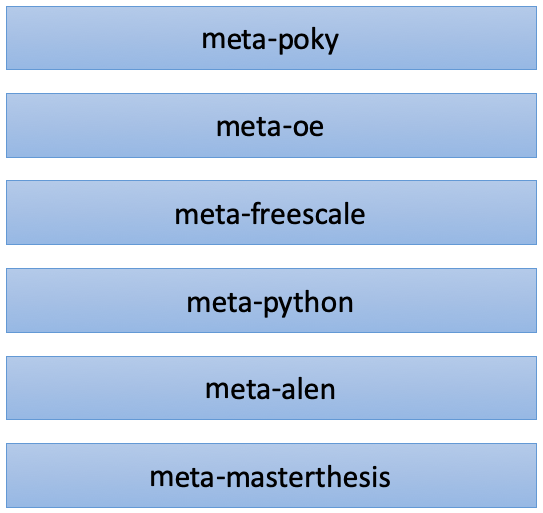
\includegraphics[width=.4\textwidth]{images/yocto_layer.png}
	\caption{\textit{Yocto Layer}}
	\label{fig:yocto_layer}
\end{figure}

\subsection{Verkabelung im Fahrzeug}

Damit die ALEN Zugriff auf den CAN-Bus bekommt, muss sie an ihn angeschlossen werden. Hierfür kommt prinzipiell jede beliebige Stelle der Linie im Auto infrage. Zum Beispiel kann dazu das CAN-Gateway angezapft werden oder ein T-Stück an den zwei Kabeln irgendwo in der Nähe des Fahrerraums. Hinter dem Lenkrad ist deshalb eine sehr gute Position, da es mit dem Antriebsstrang verbunden ist und viel Platz für die Montage bietet. Der Kabelbaum wird daher aufgetrennt und jeweils eine abzweigende Leitung an den CAN-High und CAN-Low gelötet. Bevor diese in eine RJ11 Buchse gesteckt werden, müssen sie gegen Reflexionen mit einem 120\si{\ohm} Widerstand terminiert werden. Für die Spannungsversorgung wird der 12V Zigarettenanzünder mit einem Adapter verwendet. Abbildung \ref{fig:alen_wireing} zeigt den schematischen Aufbau.

\begin{figure}[htbp]
	\centering
    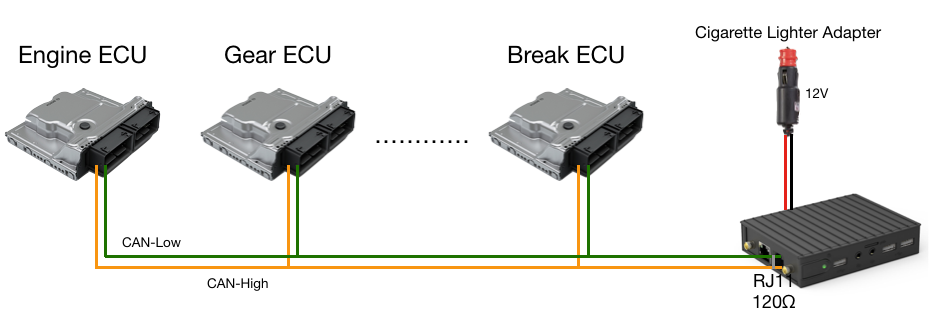
\includegraphics[width=.6\textwidth]{images/alen_wireing.png}
	\caption{ALEN Verkabelung}
	\label{fig:alen_wireing}
\end{figure}

\section{Softwarekomponenten}
\label{sec:software_compontens}

Die Architektur des Systems zeigt bereits auf, welche Softwarekomponenten auf der CCU zu realisieren sind. Diese sind in der folgenden Liste angeführt und in weiterer Folge im Detail erklärt.

\begin{enumerate}
    \item \textbf{CAN-Logger} zeichnet CAN-Nachrichten der Fahrwerks-CAN-Linie in fast-Echtzeit auf und speichert sie in MDF-Dateien ab.
    \item \textbf{Data-Preprocessor} bereitet die Daten für das \textit{Machine Learning} Model auf und speichert sie in HDF5-Dateien ab.
    \item \textbf{ML-Model Trainer} erstellt ein \textit{Machine Learning} Model mit einem \textit{Random Forest Classifier} und trainiert es mit den abgespeicherten Fahrerprofilen.
    \item \textbf{ML-Model Predictor} nimmt neue CAN-Dateien entgegen und klassifiziert die Datenpunkte mit dem ML-Model.
    \item \textbf{Result Presenter} sendet eine Benachrichtigung an den Fahrzeughalter, wenn eine gewisse Genauigkeit bei ausreichend Datenpunkten erzielt wird.
\end{enumerate}

\subsection{CAN-Logger}
\label{sec:can_logger}

Der Eintrittspunkt vom Fahrzeug zur ALEN ist über die CAN Schnittstelle. Bevor die CAN-Daten überhaupt verarbeitet werden können, muss es dem Betriebssystem möglich sein am Bus teilnehmen zu können. Es braucht auf der Netzwerkebene ein Interface und darüberliegend einen Treiber. Dies wird vom Kernel über das \textit{SocketCAN} Modul bereitgestellt \cite{kleine2012}. Es ist eine \textit{Open-Source} Sammlung aus einer Implementierung des CAN-Protokolls, Linux Treiber und einer CAN-Socket API. Das ermöglicht eine ähnliche Handhabung wie mit dem TCP/IP Protokoll-Stack, sodass sich Anwendungen gewöhnlich auf ein CAN-Interface mit einem Socket verbinden und Nachrichten empfangen, sowie senden können.

So verfährt auch der \textit{CAN-Logger}, dessen Aufgabe es ist, relevante Nachrichten vom Bus mitzulesen und abzuspeichern. Die Software ist in der Programmiersprache \textit{Go} entwickelt, da von \textit{Bosch} einige Bibliotheken für das Aufzeichnen und Verarbeiten von CAN-Daten für Linux-Systeme existieren. Durch eine Socketverbindung auf das CAN-Interface wird jede einzelne Botschaft als \textit{Raw Dataframe} eingelesen. Erst durch den Abgleich des \textit{Message Identifiers} mit der abgelegten CAN-Matrix kann die Nachricht interpretiert werden. Die Umrechnung der Werte in den dazugehörigen physikalischen Größen wird von einer \textit{Library} mithilfe der Spezifikationen von der DBC-Datei erledigt. Aus Performancegründen werden nicht alle Nachrichten von der CAN-Linie verarbeitet. In der Datenbank sind nur jene inkludiert, die für diese Anwendung relevant sind. Die originale Datei beinhaltet nämlich für den Antriebsstrang etwa 270 Nachrichten mit 1500 Signalen. Dies gilt konkret für einen VW Golf 7, jedoch unterscheidet es sich kaum zu anderen Fahrzeugtypen. Die tatsächlichen relevanten Signale können aus den Erkenntnissen des vorherigen Kapitels entnommen werden. Das Resultat der \textit{Feature Selection} aus \ref{sec:feature_selection} hat gezeigt, dass nur 21 \textit{Features} für ein aussagekräftiges ML-Ergebnis ausreichend sind. Welche das sind, sind in der Abbildung \ref{fig:feature_perm_importance} ersichtlich. Diese sind aus den folgenden acht Signalen errechnet und in sechs CAN-Botschaften enthalten.

\textit{Bremsdruck}, \textit{Geschwindigkeit}, \textit{Motordrehzahl}, \textit{Fahrpedalrohwert}, \textit{Längsbeschleunigung}, \textit{Querbeschleunigung}, \textit{Lenkradwinkel}, \textit{Lenkradgeschwindigkeit}

Die DBC-Datei wird demnach auf ein minimales Subset reduziert. Neben dem angesprochenen geringeren Rechenaufwand für den \textit{CAN-Logger} selbst, sinkt der notwendige Speicherbedarf und auch die darauffolgenden SW-Komponenten werden entlastet. Sie müssen nur die Signale verarbeiten, welche für die \textit{Machine Learning} Anwendung sinnvoll sind. Beim Erhalt einer CAN-Nachricht legt die Software die umgerechneten Werte mit einem in Nanosekunden aufgelösten Zeitstempel in den Speicher ab und nach jeweils einer Minute werden alle gesammelten Daten in eine MDF-Datei gespeichert.

\subsection{Data-Preprocessor}
\label{sec:data_preprocessor}

Das Resultat dieser Komponente sollen Daten sein, die direkt für das \textit{Machine Learning Model} verwertbar sind. Das bedeutet, dass sie das gleiche Format und die Struktur haben müssen, wie jene mit denen das \textit{Model} trainiert wurde. Da für den RF-Algorithmus durch das 4. Kapitel bereits optimale Parameter mit den vorhanden Datensätzen bekannt sind, werden die neuen Daten auf die gleiche Struktur gebracht. Des weiteren wird ebenfalls \textit{Python} mit den verwendeten Modulen eingesetzt.

Hierfür überwacht der \textit{Data-Preprocessor} das Verzeichnis in dem der \textit{CAN-Logger} die Dateien abspeichert und wenn eine neue hinzukommt, wird sie eingelesen. Der erste Schritt ist, die Frequenzen aller Signale anzugleichen. Wie in Abschnitt \ref{sec:data_preprocessing} beschrieben beträgt sie 0.5Hz. Danach gilt es die gewünschten 21 \textit{Features} aus den Signalen zu bekommen. Je nach Signal werden Minimal-, Maximal-, Durchschnittswert, Standardabweichung und Median berechnet. Der nächste Schritt löscht alle Datenreihen, wo sich das Auto im Stillstand, zum Beispiel bei einer roten Ampel, befindet. Diese Daten können nichts zur Klassifizierung beitragen, da sie keine Aussagekraft haben. Als letztes erfolgt das Speichern der neuen Datensätze in HDF5 Dateien.

\subsection{ML-Model Trainer}
\label{sec:ml_model_trainer}

Der \textit{ML-Model Trainer} ist die erste Softwareinstanz, welche nach dem Hochfahren der ALEN gestartet wird. Die Funktion dessen ist, einen \textit{Random Forest Classifier} zu erstellen und mit abgelegten Fahrerprofilen zu trainieren. Auch hier kommt \textit{Scikit-Learn} zum Einsatz und die Parameter werden wie erwähnt von den Optimierungsresultaten übernommen. Die Profile sind durch den \textit{CAN-Logger} aufgezeichnete und vom \textit{Data-Preprocessor} gefilterte Daten von jeweils einer Person. Dadurch ist sichergestellt, dass sie die gleichen Eigenschaften wie die zu klassifizierenden Daten haben und zu 100\% zuordenbar sind.

\subsection{ML-Model Predictor}
\label{sec:ml_model_predictor}

Nach dem \textit{Data-Preprocessor} ist der \textit{ML-Model Predictor} geschaltet. Er überwacht wiederum das Verzeichnis, indem die HDF5 Dateien nach der Vorverarbeitung gespeichert werden. Kommt eine neue Messdatei hinzu, wird sie eingelesen und auf ihre Korrektheit validiert. Darunter zählt die Überprüfung, ob alle Datenreihen inkludiert sind und ob alle Signale zu jedem gegebenen Zeitpunkt einen Wert haben. Ergeben sich Inkonsistenzen, wird die Datei übersprungen. So wird vermieden, dass es zu Verfälschungen während der Analyse kommt und dadurch auch zu keiner Missklassifizierung. Hat die Datei die erwartete Struktur, wird sie zu den in dieser gestarteten Fahrt bereits aufgenommen Daten hinzugefügt und in das erstellte Ml-Modell eingespeist. Das Ergebnis ist eine Reihe an Werten, welche jeweils die prognostizierte Klasse sind. Die Einträge repräsentieren somit den klassifizierten Fahrer für die entsprechende Eingabe-Datenreihe. Der nächste Schritt ist die Auswertung, um welche Fahrerin es sich dabei handelt. Als erstes wird die Häufigkeit der vorhandenen Klassen (1 bis 4) ermittelt. Danach können mehrere Methoden zur Evaluierung eingesetzt werden.

\subsubsection{Grenzwert}

Eine Möglichkeit ist folgende. Übersteigt der prozentuale Anteil eines Fahrers eine gewisse Grenze, ist mit dieser Wahrscheinlichkeit das der Fahrer. Zum Beispiel sind nach fünf Minuten Fahrzeit 150 Datenreihen (30 pro Minute, 0,5Hz) verfügbar. Das Resultat des \textit{Random Forest Models} hat ergeben, dass etwa sieben Messpunkte (5\%) zu Fahrer \textit{1} gehören könnten, 15 (10\%) zu Fahrer \textit{2} und über 22 (15\%) zum Fahrprofil \textit{3}. 105 (70\%) Eingabedaten deuten jedoch auf Fahrer \textit{4} hin. Muss die Grenze von 70\% erreicht werden, um eine Fahrer identifizieren zu können, würde das Endergebnis der Klassifizierung diesen Fahrer bevorzugen.

\subsubsection{Differenz}
\label{sec:identification_difference}

Angenommen der \textit{Output} des Modells ist nicht so eindeutig und ergibt jeweils für Fahrerin \textit{1} und \textit{2} 5\%, für Fahrerin \textit{2} 30\% und 60\% für Fahrerin \textit{4}. Nach dem ersten Ansatz wäre hier keine eindeutige Identifikation möglich. Um trotzdem auf ein zuverlässiges Ergebnis zu kommen, kann eine andere Herangehensweise angewendet werden. Sie betrachtet nur die zwei am häufigsten vorkommenden Klassen - in diesem Fall Fahrerin \textit{3} und \textit{4} - und bildet davon die Differenz. Ist diese groß genug, kann es für eine ausreichende Identifikation genügen. Hier bietet sich der Wert 30 an (Kriterium 1). Dadurch ist auch sichergestellt, dass die Klasse mit dem höchsten Anteil mindestens 50\% hat (Kriterium 2). Für ein besseres Verständnis sind unten Beispiele angeführt, welche alle für die Fahrerin \textit{4} sprechen.

\begin{table*}[htbp]
    \centering
    \caption{Beispiel Differenzansatz für Fahrerin 1 - 4}
    \label{tab:differencial_approach}
    \begin{tabular}{|l|l|l|l|l||l|l|l|}
        \hline
         & \textit{P(1)} & \textit{P(2)} & \textit{P(3)} & \textit{P(4)} & Kriterium 1 & Kriterium 2 & Ergebnis \\
        \hline
        1. min & 0\% & 0\% & 30\% & 70\% & 70 - 30 $\geq$ 30 & 70 $\geq$ 50 & \textit{P(4)} \\
        2. min & 10\% & 20\% & 10\% & 60\% & 60 - 20 $\geq$ 30 & 60 $\geq$ 50 & \textit{P(4)} \\
        3. min & 20\% & 20\% & 20\% & 50\% & 50 - 20 $\geq$ 30 & 50 $\geq$ 50 & \textit{P(4)} \\
        4. min & 10\% & 10\% & 30\% & 60\% & 60 - 30 $\geq$ 30 & 60 $\geq$ 50 & \textit{P(4)} \\
        5. min & 0\% & 10\% & 20\% & 75\% & 75 - 20 $\geq$ 30 & 75 $\geq$ 50 & \textit{P(4)} \\
        \hline
  \end{tabular}
\end{table*}

\subsubsection{Zeitliche Veränderung}

Weiters kann auch die zeitliche Veränderung der Häufigkeiten analysiert werden. Das ist hilfreich, wenn sich die Individualität der Personen erst nach den ersten Fahrminuten für das ML-Modell sichtbar macht. So müssen nicht mehr Daten als nötig gesammelt werden, um die nicht-eindeutigen zu kompensieren. Die Methode analysiert jede Datei für sich und speichert die Zwischenergebnisse ab. Danach wird jeweils das Delta berechnet und der Maximalwert bestimmt. Ist das Delta positiv und übersteigt sowie der Maximalwert eine gewisse Grenze, kann der Lenker identifiziert werden. Die Tabelle \ref{tab:time_dependet_analyzis} zeigt ein Beispiel, bei dem die ersten beiden Ansätze noch keinen Fahrer eindeutig identifizieren könnten. Im Durchschnitt sind 45\% der Daten auf Fahrer \textit{4} klassifiziert worden, was zu wenig ist. Die zeitbasierte Veränderung spricht jedoch klar dafür.

\begin{table*}[htbp]
    \centering
    \caption{Beispiel Zeitliche Veränderung der Wahrscheinlichkeiten für Fahrer 1 - 4}
    \label{tab:time_dependet_analyzis}
    \begin{tabular}{|l|l|l|l|l|}
        \hline
         & \textit{P(1)} & \textit{P(2)} & \textit{P(3)} & \textit{P(4)} \\
        \hline
        1. min & 20\% & 20\% & 30\% & 30\% \\
        2. min & 20\% & 25\% & 25\% & 30\% \\
        3. min & 10\% & 20\% & 30\% & 40\% \\
        4. min & 0\% & 20\% & 25\% & 55\% \\
        5. min & 0\% & 10\% & 20\% & 75\% \\
        \hline
        $\diameter$ & 10\% & 18\% & 26\% & 45\% \\
        \hline
        $\Delta$ & -20\% & -10\% & -15\% & +45\% \\
        \hline
        max & 20\% & 25\% & 30\% & 75\% \\
        \hline
  \end{tabular}
\end{table*}

Um eine Methode auswählen zu können, welche letztendlich für das System zum Einsatz kommt, wurde jede implementiert und mit den Testdaten mehrmals evaluiert. Das hat ergeben, dass sich der zweite Ansatz am besten hierfür eignet. Im Gegensatz zum ersten ist er flexibler und findet schneller den korrekten Fahrerin. Zusätzlich hat sich herausgestellt, dass bereits nach den ersten Minuten das Fahrverhalten der Testfahrer unterscheidbar ist. Daher ist die letzte Implementierung nicht anwendbar, da sich das Delta nicht merklich verändert. Als Absicherung kann des Weiteren die Anwendung so konfiguriert werden, dass die identifizierte Fahrerin erst dann bestätigt ist, wenn sich das Ergebnis bei den darauffolgenden Durchläufen nicht mehr ändert. Umso länger abgewartet wird, desto sicherer gilt es, aber umso länger muss mit der darauf basierenden Aktion gewartet werden. Es gilt daher das richtige Verhältnis zwischen der Identifikationszeit und wie lang auf die Umsetzung der Aktion gewartet werden darf, zu finden. Beispielsweise macht es für individuelle Anpassungen keinen Sinn länger als zehn Minuten zu warten, aber der Eintrag ins digitale Fahrtenbuch kann auch erst am Ende der Fahrt erfolgen.

\subsection{Result Presenter}

Wie die Aktion nun ausgelöst wird, übernimmt die Komponente \textit{Result Presenter}. Je nach Service kann dies auf unterschiedlichen Kommunikationswegen geschehen. Soll das Auto selbst darauf reagieren, zum Beispiel das Anzeigen der zuletzt ausgewählten Ziele im Navigationssystem, kann die Information wieder zurück über den CAN-Bus übertragen werden. Wird hingegen nach einer gewissen Zeit gar kein Fahrer erkannt, womöglich also eine unautorisierte Person, ist es denkbar eine SMS an den Fahrzeughalter zu versenden. Da die ALEN ein GSM Modul mit SIM-Karte integriert hat, ist es ohne weiteres umsetzbar. Über die Internetverbindung können auch Dienste des Herstellers oder von Drittanbietern angebunden werden, welche ein REST API zur Verfügung stellen. Es hängt demnach sehr stark davon ab, was mit der Erkenntnis passieren soll.

\subsection{Sequenzdiagramm}

Das folgende Diagramm (Abbildung \ref{fig:sw_components_sequence}) zeigt die Funktionen der einzelnen Komponenten. Dadurch, dass fast kein tatsächlicher Nachrichtenaustausch stattfindet, sondern meist nur Dateien abgelegt werden, gibt es wenige direkte Querverbindungen. Nach dem Hochfahren der ALEN, was in etwa zehn Sekunden dauert, wird zuerst der \textit{CAN-Logger} und der \textit{ML-Model Trainer} gestartet. Danach folgt der \textit{Data-Preprocessor}, der \textit{ML-Model Predictor} und der \textit{Result Presenter}. Obwohl es aus logischer Sicht unabhängige und alleinstehende Komponenten sind, werden die letzten drei bei der Umsetzung zusammengeführt. Das hat den Grund, dass einerseits die Klassifizierungslogik das zuvor erstellte Modell benötigt und andererseits unmittelbar danach die Funktion zum Weiterleiten der Information, welche kein großes Ausmaß annimmt, aufgerufen wird.

\begin{figure}[htbp]
	\centering
    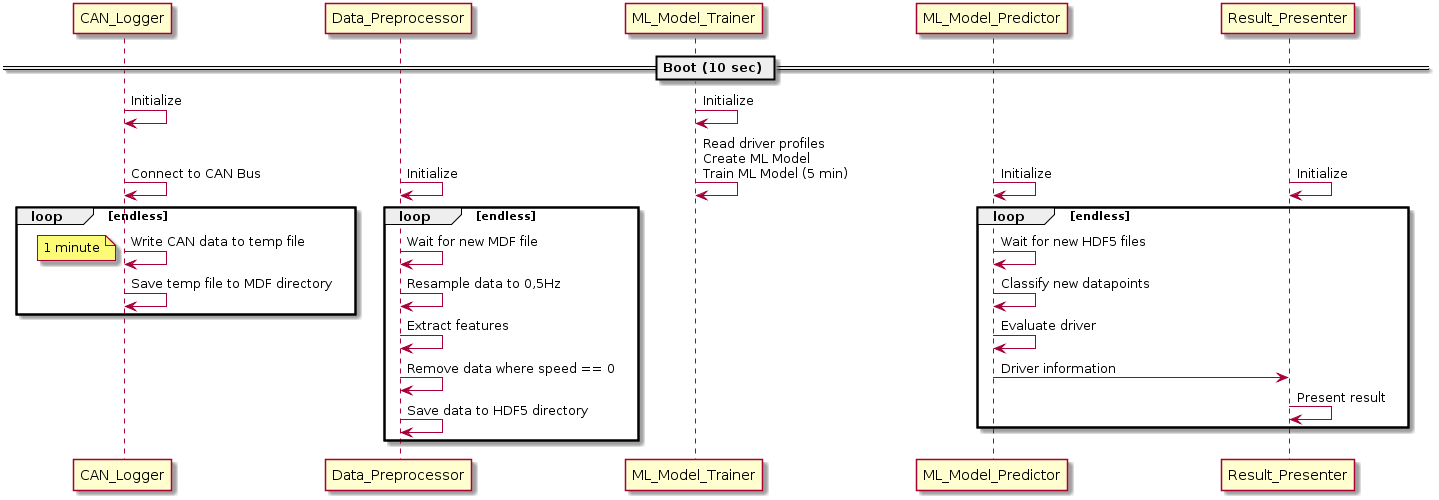
\includegraphics[width=\textwidth]{images/sw_components_sequence.png}
	\caption{Sequenzdiagramm Software Komponenten}
	\label{fig:sw_components_sequence}
\end{figure}

\section{Simulation}
\label{sec:simulation}

Das letzte Ziel der Masterarbeit ist, das entwickelte System in ein Fahrzeug zu integrieren. Da jedoch das Unternehmen, mit dem es umgesetzt wird, leider kein entsprechendes bereitstellen kann, muss es simuliert werden. Normalerweise würden vier Personen mehrere Testfahrten durchführen, um ein Profil anzulegen. Bei weiteren Fahrten könnte das System in Folge dessen erprobt werden. Da dies eben nicht möglich ist, dienen hierzu zufällige vier der vorhandenen Datensätze. Für diesen Zweck werden die Start- und Endzeitpunkte jeder Fahrt extrahiert und abgespeichert. Im Durchschnitt enthält ein Datensatz 46 Fahrten, von dem per Zufall zehn Fahrten entnommen werden, sodass diese nicht mehr in der originalen Datei enthalten sind. Das ist insofern wichtig, damit der \textit{Random Forest Classifier} die Testdaten nicht kennt und das Ergebnis verfälscht. Nach diesem Vorgang existiert daher pro Fahrer ein Trainingsset aus ungefähr 36 Fahrten und ein Testset aus zehn. Werden die Daten für einen Test, wie er zum Beispiel in Abschnitt \ref{chap:set_up} oder \ref{chap:optimization} gemacht wurde, verwendet, kommt eine Genauigkeit des Modells von ca. 94\% heraus. Die Steigerung erklärt sich durch die geringere Anzahl an Fahrerprofilen.

Um die Simulation so realgetreu wie möglich zu implementieren, wird nur der \textit{CAN-Logger} ersetzt. Stattdessen werden von einem eigenen Programm (\textit{MDF-Simulator}) MDF Dateien in das Verzeichnis abgelegt, aus dem der \textit{Data-Preprocessor} diese bezieht. Bei den MDF Dateien handelt es sich um jene, welche im \ref{chap:set_up}. Kapitel vorgestellt wurden und bilden das Testset. Da sie jeweils eine Minute an Fahrtzeit beinhalten, wird auch immer eine Datei nach einer Minute in das dezidierte Verzeichnis hinzugefügt. Die Reihenfolge ist dabei chronologisch, beginnend mit der ersten Minute einer Fahrt. Durch die neue Komponente wird lediglich das erste Glied (CAN-Bus und -\textit{Logger}) simuliert. Für die restlichen Software-Teile hat es keine Auswirkung. Da das ganze System auch auf der ALEN in Betrieb genommen wird, ergeben sich fast reale Bedingungen und die daraus resultierenden Ergebnisse haben eine hohe Aussagekraft.

Zusammenfassend lässt sich die Simulationsumgebung folgendermaßen beschreiben: Die Softwarekomponenten werden wie beschrieben implementiert, lediglich der \textit{CAN-Logger} wird durch den \textit{MDF-Simulator} ersetzt. Für die Identifikation eines Lenkers kommt der \textit{Differenz}-Ansatz um Einsatz. Als Fahrerprofile werden vier der vorhandenen Datensätze herangezogen, bei denen zehn Fahrten gelöscht werden. Die original MDF Dateien von den gelöschten dienen hierzu als Eingabedaten. Bei einem Testdurchlauf verwendet der \textit{MDF-Simulator} immer nur Dateien von einer Fahrerin, da es darum geht, nur einen zu identifizieren. Zur Benachrichtigung wird ein SMS-Versand mit dem integrierten Modul und SIM-Karte umgesetzt.

\subsection{Fahrererkennung}
\label{sec:driver_identification}

Das Listing \ref{lst:sw_rf} zeigt einen Ausschnitt der letzten drei genannten Komponenten. Von Zeile zwei bis elf werden die abgelegten Fahrerprofile geladen, ein \textit{Random Forest Classifier} erstellt und trainiert. Ab Zeile dreizehn beginnt die Logik für die Fahrererkennung. Es beinhaltet das Einlesen neuer Messdaten sowie die Klassifizierung durch das ML-Modell. Danach werden die Häufigkeiten der Klassen gezählt und die zwei am meisten vorkommenden ermittelt. Anschließend wird die Überprüfung nach dem \textit{Differenz}-Ansatz durchgeführt und schlussendlich eine SMS Versand, wenn der Fahrer oft genug bestätigt wurde.

\begin{lstlisting}[frame=lines, caption=Ausschnitt Fahreridentifikation, captionpos=b, label = lst:sw_rf, numbers=left, language=Python, showstringspaces=false, basicstyle=\footnotesize]
    [...]
    # ML Model Trainer
    profiles = get_profiles(config["profile_dir"])
    features = config["features"][:21]
    X = profiles[features].values
    Y = profiles["class"]

    clf = RandomForestClassifier(n_estimators=300, min_samples_leaf=1, min_samples_split=3, criterion="gini", max_depth=None)
    clf.fit(X, Y)

    # ML-Model Predictor
    all_data = []
    while True:
        data = []
        for file in os.listdir(config["input_dir"]):
            df = pd.read_hdf(os.path.join(config["input_dir"], file))
            data.append(df)

        all_data = all_data + data

        pdata = pd.concat(all_data, sort=False)
        pdata = pdata.values

        pred = clf.predict(pdata)

        ids, counts = np.unique(pred, return_counts=True)
        ids = dict(zip(ids, counts))
        first = {"id": None, "count": 0}
        second = {"id": None, "count": 0}
        for id in t:
            c = ids[id]
            if c > first["count"]:
                first["count"] = c
                first["id"] = id
            elif c > second["count"]:
                second["count"] = c
                second["id"] = id

        first_conf = first["count"] / len(pred)
        second_conf = second["count"] / len(pred)
        diff = first_conf - second_conf
        if diff >= 0.30 and first_conf >= 0.50:
            if confirmed_id == first["id"]:
                confirmation_count += 1
            else:
                confirmed_id = first["id"]
                confirmation_count = 1

        if confirmation_count == config["confirmation_count"]:
            # Result Presenter
            send_SMS("\nDriver with id %s is driving" % first["id"], config["number"])
            break
    [...]
\end{lstlisting}

\subsection{Ergebnisse}

In diesem Abschnitt werden kurz die Ergebnisse der Simulation auf der ALEN präsentiert. Bis das \textit{Machine Learning Model} fertig trainiert ist, vergehen ca. fünf Minuten bei vier Profilen mit allen verfügbaren Fahrten (exklusive zehn). Aufgrund dessen beträgt die Anzahl wie oft eine Fahrerin hintereinander identifiziert werden muss fünf. Es liegen nämlich nachdem das Trainieren des Modells abgeschlossen ist, bereits fünf Dateien mit jeweils einer Minute an Fahrzeit vor. Für das Klassifizieren einer neuen Datei benötigt das Gerät unter eine Sekunde.

Bei einem Testdurchlauf wurde jeweils eine Fahrt herangezogen und festgestellt wie viele Minuten nötig sind, bis der Fahrer korrekt identifiziert wird. Um ein fundierteres Ergebnis zu bekommen, ist der Vorgang öfters mit permutierten Trainings- und Testfahrten durchlaufen worden. Der ganze Vorgang wurde auch mit allen vier Fahrern vollzogen. Dabei ist das Folgende herausgekommen.

\begin{itemize}
    \item Der Algorithmus hat mit einer Wahrscheinlichkeit von 97\% den Fahrer korrekt identifiziert.
    \item Lediglich drei Fahrten wurden falsch zugeordnet.
    \item Nur eine Fahrt konnte gar nicht zugeordnet werden.
    \item Für eine Identifikation wurden im Schnitt 5,73 Minuten an Fahrzeit benötigt.
\end{itemize}

%----------------------------------------------------------------
%
%  File    :  discussion.tex
%
%  Authors :  David Lechner, FH Campus Wien, Austria
%
%  Created :  10 Oct 2019
%
%  Changed :  10 Oct 2019
%
%----------------------------------------------------------------


\chapter{Diskussion}
\label{chap:discussion}

Das letzte Kapitel vor der Zusammenfassung präsentiert die erzielten Ergebnisse der Masterarbeit und diskutiert die Erkenntnisse. Die Gliederung spiegelt die behandelten Forschungsfragen. Des Weiteren wird ein Ausblick über weiterführende Tätigkeiten gegeben.

\section{Validierung der Methoden}

Im Abschnitt \ref{sec:related_work} wurden vier Paper vorgestellt, welche sich mit dem gleichen Thema - Fahreridentifikation basierend am Fahrverhalten - beschäftigen. Diese haben hauptsächlich den \textit{Machine Learning} Algorithmus \textit{Random Forest} verwendet und damit gute Resultate erzielen können (teilweise über 85\%). Es wurde jedoch sehr wenig über die Struktur, Eigenschaften und Herkunft der Daten erwähnt. Daher war die erste Frage: Sind die existierenden Methoden mit den vorhandenen Daten valide? Kapitel \ref{chap:set_up} hat gezeigt, dass dies zutrifft, da bei einem ersten Versuch eine Genauigkeit des Modells von 85\% herausgekommen ist. Weitere Durchläufe haben hingegen eine hohe Schwankungsbreite - von 78,66\% bis 92,53\% - ergeben. Das lässt sich auf zwei Gründe zurückführen. In Sektion \ref{sec:feature_optimization} bei der \textit{Feature}-Analyse wurde entdeckt, dass das Signal \textit{Gangposition} Unregelmäßigkeiten aufweist. Bei fünf von neun Datensets ist der Wert durchgehend \textit{14}. Die guten Ergebnisse (über 90\%) können zum Teil daher kommen, dass das Trainings- und Testset gleichverteilt Datenpunkte mit und ohne Gangposition \textit{14} haben. Dadurch bekommt, wie in Abbildung \ref{fig:feature_importance} gezeigt, das \textit{Feature} eine große Bedeutung und hilft ungemein bei der Klassifizierung. Der zweite Grund ist, dass die Auswahl der Daten einen Einfluss auf die Genauigkeit haben. Befinden sich viele Autobahnkilometer, welche wenig Individualität aufweisen und schwerer zuordenbar sind, unter den Sets, sinkt die Trefferquote. Das Gegenteil tritt bei vielen Datenpunkten von Lenk- oder Bremsmanöver auf, die Trefferquote steigt.

Das \ref{chap:set_up}. Kapitel hat die vorliegenden Daten beschrieben. Im Gegensatz zu \cite{Gahr2018} sind sie direkt von mehreren CAN-Linien abgegriffen worden und nicht über den Diagnostik-Port (OBD II). Das bringt einige Vorteile. Zum Beispiel sind aufgrund dessen alle vorhandenen Signale am Bus verfügbar. Alleine am Fahrwerks-CAN sind bis zu 1500 und am Komfort-CAN über 2500 Signale vorhanden. Je nach Hardwarekapazitäten und Fahrzeugmodell können auch noch mehrere CAN-Linien miteinbezogen werden. Damit wird das ML-Modell genauer und aussagekräftiger, wenn es mehr Daten zum Verarbeiten gibt. Währenddessen über den OBD II Port \cite{SAEII} laut Spezifikation maximal 196 Signale übertragen werden. Hier handelt es sich meist auch nur um verschiedenen Abgaswerte, Fehlerhistorie und Temperaturen. Hersteller können zudem noch weitere Signale in die Schnittstelle implementieren, welche aber nicht spezifiziert sind. Um die Werte über OBD II auslesen zu können, muss ein Dongle eingesetzt werden, der in einen dezidierten Anschluss, meist versetzt unterhalb des Lenkrads, eingesteckt wird. Er hat das OBD Protokoll implementiert und kann die Signale auswerten und in die physikalische Einheit umrechnen \cite{OBD20}. Für die Weiterverarbeitung wird gewöhnlich eine Bluetooth-Verbindung zu einem weiteren Gerät (z.B. Smartphone) benötigt. Für diese Anwendung wäre die ALEN notwendig, die die Daten empfängt und mit dem \textit{Machine Learning} Algorithmus klassifiziert. Durch den OBD II Dongle ergeben sich zusätzlich einige Angriffsvektoren, mithilfe dieser die Privatsphäre verletzt, Eigentum beschädigt und sogar Leib und Leben gefährdet werden könnte. Forscher haben hierzu 77 am Markt verfügbare Dongles getestet und sind zum Entschluss gekommen, dass alle mindestens zwei Schwachstellen enthalten \cite{USENIX20}. Beispielsweise sind keine Authentifizierungsmethoden realisiert, lassen das Extrahieren der Firmware ohne Sicherheitsmechanismus zu oder senden CAN-Nachrichten am Bus ohne jegliche Validierung. Das Abgreifen direkt vom Bus ist daher die klar bessere Methode und bietet mehr Signale, bessere Sicherheit und Schutz der Privatsphäre.

\section{Optimierung}

Bei der Beantwortung der zweiten Forschungsfrage wurde versucht, den \textit{Random Forest} Algorithmus zu optimieren. Im ersten Schritt sind die Parameter analysiert worden. Dabei hat sich herausgestellt, dass die Standardwerte bereits sehr gute Ergebnisse liefern. Selbst nach 16128 Durchläufen, bei denen jede mögliche Kombination der Parameter überprüft wurde, konnte lediglich eine Verbesserung um fast ein Prozent erzielt werden. Auffallend war, dass eine Veränderung des Wertes bei dem Parameter \textit{criterion} - von \textit{gini} auf \textit{entropy} - zwar keine Auswirkung auf die Trefferquote gehabt hat, jedoch sich die Durchlaufzeit erheblich vergrößert hat, nämlich um mehr als 300\%. Der Grund hierfür ist die dahinterstehende Formel. \textit{Entropy} wird mit dem Logarithmus der Basis 2 von der Wahrscheinlichkeit berechnet, wohingegen bei der \textit{Gini Impurity} die Wahrscheinlichkeit mit sich selbst multipliziert wird (siehe \ref{sec:random_forest}). Da die Logarithmus-Funktion mehr Rechenleistung erfordert als eine Multiplikation, ist das Aufteilen eines Knotens mit \textit{entropy} langsamer.

Durch eine detailliertere Analyse der vorhanden Datensätze hat sich eines verdeutlicht: Die Daten sind das ausschlaggebendste für die \textit{Machine Learning} Anwendung. Diese Aussage wird auch immer wieder in der Literatur (\cite{Rebala2019}, \cite{Conway2012}) bestätigt. Damit ist gemeint, dass zum einen die Struktur einheitlich und bekannt und zum anderen ausreichend viele Daten erhältlich sein müssen. Gibt es beispielsweise mehrere fehlende Werte oder Unregelmäßigkeiten (siehe \textit{Gangposition}) können manche ML Algorithmen nicht zuverlässig Ergebnisse liefern. Das gleiche gilt wenn einfach zu wenig verfügbar sind. Das Regelset des Modells kann so nicht hinreichend gebildet werden, um die Vielfalt der existierenden Daten abzubilden.

Ein ML-\textit{Model} stellt in gewisser Weise eine \textit{Blackbox} dar, da nicht ohne einer näheren Untersuchung erkennbar ist, auf Grund welcher Daten eine Entscheidung getroffen wird. Diese Erfahrung hat auch der Autor von \cite{Gahr2019} gemacht, der ebenfalls den Lenker anhand von CAN- und Smartphone-Daten identifizieren wollte. Er hat das Modell mit allen zugänglichen Daten trainiert, darunter auch Längen- und Breitengrade des GPS-Moduls. Der \textit{Classifier} hat am Ende nicht basierend am Fahrverhalten Datenpunkte zugeordnet, sondern alleine mittels den GPS-Daten. In Abschnitt \ref{sec:feature_importance} wurde ähnliches aufgezeigt. Mit Hilfe der integrierten \textit{Feature Importance} des \textit{Random Forest}s ist bemerkt worden, dass es beim Signal \textit{Gangposition} keine durchgängigen Werte gibt. Der Missstand wurde bereits oben erläutert und bekräftigt die genannte These, dass die Daten vor dem Einsatz mit \textit{Machine Learning} genauestens analysiert und validiert werden müssen. Das verhindert eine falsche Vorgehensweise des ML-Modells als \textit{Blackbox}.

\section{Dauer der Trainings- und Identifikationsphase}

Im Zuge der Optimierungen und der Integration wurde auch die Fragestellung behandelt, wie viele Trainingsdaten vonnöten sind, um mindestens 85\% Genauigkeit des \textit{Models} zu erreichen. Des Weiteren war die Frage, wie lang eine Person fahren muss, damit sie zu 85\% identifiziert werden kann. Hier kann keine pauschale Antwort gegeben werden, da viele Faktoren Einfluss darauf nehmen. Mitsicherheit die maßgeblichsten davon sind die Anzahl an Fahrprofilen in einem Set und welche Daten ausgewählt werden. Die Abbildungen \ref{fig:train_duration_shuffle} und \ref{fig:train_duration_start} zeigen den Unterschied zwischen einer zufälligen und chronologischen Auswahl. Bei ersteren ist die maximale Genauigkeit mit 40 Minuten Trainingszeit pro Fahrer bei etwa 75\% gelegen. Sind die Daten jeweils nach Fahrtbeginn für die Trainingsphase herangezogen worden, wurde nach ca. 15 Minuten knapp 86\% erreicht. Mit der Zufallsauswahl konnte das Ziel somit nicht erreicht werden. Das bestätigt die Annahme, dass Daten am Beginn einer Fahrt, wo mehrere Lenk- und Bremsmanöver stattfinden, eine höhere Individualität aufweisen und dadurch besser zu klassifizieren sind. Die beschriebenen Tests sind mit neun Fahrprofilen durchgeführt worden. Während der Integration hat ein Test mit nur vier eine Genauigkeit von 94\% ergeben. Das beweist, dass allein die Reduktion auf eine geringere Anzahl einen großen Einfluss hat.

Für die Dauer der Identifikationsphase gilt ebenso das gleiche. Da sich das Kapitel \textit{Optimierung} an erster Stelle auf die allgemeine Verbesserung des Modells konzentriert hat, ist dieser Aspekt nicht beleuchtet worden. Es liegen daher keine Ergebnisse für ein Modell mit neun Profilen vor. Das vorherige Kapitel ist jedoch explizit auf die Fragestellung eingegangen. Allerdings kann wieder keine pauschale Aussage getroffen werden, da ein paar Gegebenheiten vorausgesetzt waren. Zum einen sind im ML-Modell nur vier Datensätze inkludiert und zum anderen gibt es eine Einschränkung durch die Zeit die benötigt wird, um den \textit{Random Forest Classifier} zu trainieren. Des Weiteren ist die Art der Identifizierung durch den eingesetzten Algorithmus (siehe \ref{sec:identification_difference}) gesteuert. So muss zum Beispiel fünfmal ($\widehat{=}$ 5 Minuten) hintereinander die gleiche Fahrerin identifiziert werden. Mehreren Tests mit verschiedenen Daten haben hierbei ergeben, dass 97\% davon im Durchschnitt nach 5,73 Minuten identifiziert sind.

\section{Integration}

Die letzte Forschungsfrage zielt auf die Integration des Systems zur Fahreridentifikation in ein Fahrzeug ab. Wie in dem Kapitel beschrieben, ist es nicht möglich gewesen, da ein tatsächliches Auto nicht zur Verfügung gestellt wurde. Stattdessen ist der CAN-Bus durch die bereits vorhandenen Daten simuliert worden. Die Beschreibungen und Ergebnisse haben gezeigt, dass dies sehr gut funktioniert hat und es auf diese Weise zu fast realen Bedingungen gekommen ist. Die ALEN als zentrale Einheit eignet sich prinzipiell gut für diesen Einsatz, da sie die notwendige Peripherie mitbringt, hat aber klar ihre Grenzen in Bezug auf \textit{Machine Learning}. So dauert es ca. fünf Minuten, bis die CCU den \textit{Random Forest Classifier} erstellt und trainiert hat. Einige Maßnahmen könnten die Zeit reduzieren. Beispielsweise kann die ALEN durch eine leistungsstärkere CCU mit sonst ähnlicher Hardwareausstattung ersetzt werden. Denkbar wäre zudem, das trainierte Modell zu speichern und bei Fahrtbeginn nur zu laden. Den Prozess komplett in die \textit{Cloud} auszulagern, erfordert das Umsetzen von weitgehenden \textit{Security}- und \textit{Privacy}-Anforderungen, da sich die persönlichen Fahrprofile nicht mehr nur lokal im Auto befinden. Weiters würde dadurch das Konzept von \textit{Edge Computing} verloren gehen. Die Vorteile davon wurden in den Grundlagen näher gebracht, hat aber eben auch einen Nachteil, nämlich der von fehlenden Ressourcen am \textit{Edge Device}, vorausgesehen.

Selbst wenn die Zeit auf ein Minimum reduziert werden könnte, würde es die Identifizierung nicht zwangsläufig beschleunigen. Sie hängt hauptsächlich vom Zweck ab und wird von der Konfiguration des \textit{ML-Model Predictor} bestimmt. Dem Serviceanbieter - sei es der OEM oder eine Drittpartei - muss klar sein, dass je kürzer die Identifikationsphase gewählt wird, desto leichter kann es zu einer Missidentifikation kommen. Es gibt durchaus Services, welche erst gegen Ende einer Fahrt die Identifikation benötigen. Zum Beispiel ist in der Einleitung das digitale Fahrtbuch besprochen worden, das vollkommen ohne jeglicher Interaktion seitens der Fahrerin auskommt. Eine Implementierung auf der ALEN wäre ohne viel Zutun möglich, da dort bereits alle Daten aufliegen. Eine weitere Einsatzmöglichkeit liegt bei \textit{Car-Sharing} Anbietern. Sie können mit Hilfe des Systems erkennen, ob wirklich die registrierte Person hinter dem Lenkrad sitzt. Diese Information genügt es auch erst am Ende zu haben. Das gleiche Prinzip lässt sich zudem bei Mietwagenunternehmen realisieren. Die Standardverträge erlauben nur einen Lenker, jede weitere kostet extra Geld (\EUR{8,50} bei \textit{Sixt} \cite{SIXT}). Die Überprüfung kann hiermit durchgeführt und bei Bedarf der Vertragszusatz automatisiert ergänzt werden.

Es gibt überdies Anwendungen, die eine schnelle Identifikation erfordern. Eine davon, die Diebstahlwarnung, wurde ebenfalls schon in der Einleitung erwähnt und in diesen Kontext gesetzt. Für die Umsetzung wäre bloß eine kleine Adaption der vorhandenen Anwendung notwendig, bei der eine zusätzliche Abfrage zu unzureichenden Klassifizierungen eingebaut wird. Nachdem mehrere Versuche Dateien korrekt zuzuordnen gescheitert sind, kann eine SMS an den Fahrzeughalter gesendet werden, die darüber informiert, dass womöglich eine nicht autorisierte Person das Fahrzeug steuert. Hier muss aber klar geprüft werden, ab wann entschieden wird, dass es sich wirklich um einen unbekannten Fahrer handelt und nicht um einen bekannten, der noch nicht identifiziert wurde.

Durch die Ergebnisse des letzten Kapitels ist davon auszugehen, dass ein paar Minuten an Fahrzeit benötigt werden, damit eine Lenkerin ausreichend erkannt wird. Aus diesem Grund sind einige Services nicht umsetzbar. Allen voran jene, welche unmittelbar nach Fahrtbeginn in Kraft treten würden. Das automatische Einstellen des bevorzugten Radiosenders oder das Einrichten der Außenspiegel fallen somit weg. Ebenso die Möglichkeit, dass Fahrerabhängig bestimmte \textit{Features} de- und aktiviert werden, ist nicht vorstellbar. Das gleiche gilt für eine Drosselung der Leistung, wenn beispielsweise noch unerfahrene Personen hinter dem Steuer sitzen. Dies könnte gegebenenfalls sogar eine Gefahr darstellen, da in der Anfangszeit die volle Leistung zu einem erhöhten Unfallrisiko beiträgt.

\section{Limitierungen}

Da nur eine geringe Anzahl an Fahrdaten vorliegen, kann keine Aussage über die Genauigkeit des Systems in einer diverseren Umgebung erfolgen. Zudem fehlen CAN-Nachrichten von mehr Fahrzeugtypen, um das Modell mit den Signalen validieren zu können. Des Weiteren sind keine Informationen über Geschlecht, Altersgruppen und Dauer des Führerscheinbesitzes von den vorhandenen Fahrprofilen bekannt. Es ist daher auch unklar, ob es sich dabei um eine repräsentative Gruppe an Testpersonen handelt. Bei nur neun ist es anzunehmen. Obwohl die Simulation den realen Bedingungen sehr nahe kommt, können trotzdem nicht alle Eventualitäten abgebildet werden. Das resultiert wahrscheinlich in einer Abweichung der Zuverlässigkeit der Anwendung.

\section{Ausblick}

Um das vorgestellte System zur Fahreridentifikation zu verbessern, gibt es mehrere Möglichkeiten. Neben dem \textit{Random Forest} sind in der Literatur auch andere Algorithmen zur Klassifizierung (\cite{Rebala2019}, \cite{Enev2016}) beschrieben. Bei einem Vergleich könnte sich ein anderer als performanter und genauer herausstellen. Das Modell kann zusätzlich optimiert werden, indem eine \textit{Feedback}-Schleife implementiert wird. Nach einer erfolgreichen Identifikation werden die neuen Messpunkte dem Modell als neue Trainingsdaten zur Verfügung gestellt. Dadurch lernt der \textit{Classifier} durchgehend neue Fahrsituationen. Ein anderer Ansatz wäre nur Datenpunkte herzunehmen, welche leichter zu klassifizieren sind. Kapitel \ref{chap:set_up} und \ref{chap:optimization} haben aufgezeigt, dass solche existieren. Hier stellt sich die Frage, welche Fahrmanöver eine höhere Individualität aufweisen. Die Messdateien können folglich im \textit{Data-Preprocessor} auf die relevanten Daten reduziert werden. Als Anhaltspunkt dienen hierfür die Arbeiten \cite{Gahr2018} und \cite{Hallac2016}, die sich zum Teil schon damit beschäftigt haben.

Ein weiterer Punkt ist die Anwendung mit einem echten Fahrzeug zu erproben, da dies nicht möglich war. Im Zuge dessen ist eine Überprüfung der Simulationsergebnisse möglich. Außerdem wäre es interessant zu wissen, ob sich das System durch eine manipulierte Fahrweise austricksen lässt. Dadurch kann die Stabilität getestet werden und ob die Fahrweise von einer Person nachgeahmt werden kann.

%----------------------------------------------------------------
%
%  File    :  conclusion.tex
%
%  Authors :  David Lechner, FH Campus Wien, Austria
% 
%  Created :  10 Oct 2019
% 
%  Changed :  10 Oct 2019
% 
%----------------------------------------------------------------


\chapter{Zusammenfassung}
\label{chap:conclusion}

Zusammenfassung



%% ....


% --- Verzeichnisse ------------------------------------------------------

\newpage
%\chapter{Verzeichnisse}

% --- Bibliography ------------------------------------------------------

\bibliographystyle{alpha}

% List references I definitely want in the bibliography,
% regardless of whether or not I cite them in the thesis.

\newpage
%\phantomsection
%\addcontentsline{toc}{chapter}{Literaturverzeichnis}
\addcontentsline{toc}{chapter}{Bibliography}
\bibliography{thesis}

\newpage

% --- List of Figures ----------------------------------------------------

%\newpage
%\phantomsection
%\addcontentsline{toc}{chapter}{Abbildungsverzeichnis}
\addcontentsline{toc}{chapter}{List of Figures}
\listoffigures


% --- List of Tables -----------------------------------------------------

\newpage
%\phantomsection
%\addcontentsline{toc}{chapter}{Tabellenverzeichnis}
\addcontentsline{toc}{chapter}{List of Tables}
\listoftables

% --- List of Listings -----------------------------------------------------

\newpage
%\phantomsection
\addcontentsline{toc}{chapter}{Listings}
%\lstlistoflistings

          % List of figures/tables/listings; bibliography

\appendix
%----------------------------------------------------------------
%
%  File    :  appendix.tex
%
%  Authors :  David Lechner, FH Campus Wien, Austria
% 
%  Created :  10 Oct 2019
% 
%  Changed :  10 Oct 2019
% 
%----------------------------------------------------------------

\chapter{Anhang/Ergänzende Information}
\label{chap:app}

EIGENER ANHANG

(Hier können Schaltpläne, Programme usw. eingefügt werden.)

\clearpage		   % other appendices

\end{document}
